\documentclass[a4paper,12pt]{article}
    \usepackage[utf8]{inputenc}
    \usepackage[T1]{fontenc}
    \usepackage[english]{babel}
    \usepackage{graphicx}
    \usepackage{geometry}
    \geometry{a4paper,
                 tmargin = 35mm, 
                 lmargin = 25mm,
                 rmargin = 30mm,
                 bmargin = 30mm}
    \usepackage{mathtools}
    \usepackage{amsmath}
    \usepackage{color}
    \usepackage{setspace}
    \usepackage{amsmath,amssymb}
    \usepackage{float}
    \usepackage{listings}
    
    \usepackage{indentfirst}
	\usepackage{subfig}
	    
    \renewcommand\thesection{\Roman{section}.}
    \renewcommand\thesubsection{\thesection\arabic{subsection}}
    \renewcommand\thesubsubsection{}
    
\begin{document}

\linespread{1.2}

\begin{titlepage}

	\centering
	{\scshape\LARGE ELTE Faculty of Science\par}
	\vspace{3cm}
	{\scshape\Large Classical chaotic scattering\par}
	\vspace{1cm}
	{\large\itshape Alex Olar \par}
	\vspace{3cm}
	{\large 2018 \par}

\end{titlepage}

\onehalfspacing

\begin{abstract}
	\par The problem is the following. I projectile of mass \texttt{m} moves
	in a potential \textit{V(x, y)} through space. The Newtonian equations describe
	the trajectory as:

	\begin{equation}
		\vec{F} = m\vec{a}
	\end{equation}

	\par For a given potential:

	\begin{equation}
		-\frac{\partial V}{\partial x}\hat{i} -
		\frac{\partial V}{\partial y}\hat{j} = m \frac{d^{2}\vec{x}}{dt^{2}}
	\end{equation}

	\par The given example for \textit{V(x,y)} in the book \cite{book}:

	\begin{equation}
		V(x,y) = \pm x^{2}y^{2}e^{-(x^{2}+y^{2})}
	\end{equation}

	\par However, I am planning on generalizing the algorithm to solve
	the ODEs for any given potential. On the other hand, using
	\textit{well shaped} potentials must be taken into consideration since the
	idea behind the scattering \cite{wiki} problem is modelling real world problems such as
	a pinball game, squash, nuclei and much more. So far I have taken into
	consideration the given example above and:

	\begin{equation}
		V(x,y) = \pm x^{2}e^{-(x^{2}+y^{2})}
	\end{equation}

	\par Due to symmetry reasons the potential above is the same for
	a \textit{x,y} change as it only means a different projectile direction in
	layman's term.

	\par The second order ODEs after derivation are the following
	(for the given example):

	\begin{align}
		m\frac{d^{2}x}{dt^{2}} = \mp 2y^{2}x(1-x^{2})e^{-(x^{2}+y^{2})} \\
		m\frac{d^{2}y}{dt^{2}} = \mp 2x^{2}y(1-y^{2})e^{-(x^{2}+y^{2})}
	\end{align}
\end{abstract}

\tableofcontents

\newpage

\section{Solution}

\par The solution was computed with the \textit{scipy} package and therefore
the implementation was done in python. \textit{Scipy} provides an interface
for the LSODA solver from implemented in FORTRAN that is capable of identifying
the type of the first order differential equation (stiff or non stiff) and solving
it appropriately. It is way better than a basic Runge-Kutta method and thus gives
more appropriate results and runs faster.

\lstset{language=Python}
\lstset{frame=lines}
\lstset{caption={Derivative calculations}}
\lstset{basicstyle=\footnotesize}
\begin{lstlisting}
    def scatter(X, t, m, sign):
    x, y, u, v = X
    # Hard coded potential
    dVdx = (1./m)*sign*2*y**2*x*(1-x**2)*np.exp(-(x**2+y**2))
    dVdy = (1./m)*sign*2*x**2*y*(1-y**2)*np.exp(-(x**2+y**2))
    # Derivative
    dXdt = [u, v, -dVdx, -dVdy]
    return dXdt
\end{lstlisting}

\par It can be seen how simple it is to input a differential equation. This is the
format in which the input function should have been constructed and the method from
\textit{scipy} simply solves it as:

\lstset{language=Python}
\lstset{frame=lines}
\lstset{caption={Equation solver}}
\lstset{label={lst:code_direct}}
\lstset{basicstyle=\footnotesize}
\begin{lstlisting}
    solution = eqsolver(scatter, X0, t, args=(m, sign))
\end{lstlisting}

\par Where \textbf{X0} are the initial \textit{x, y, u, v}. Since the second order
differential equations were separated as:

\begin{align*}
	I. \quad m\frac{d^{2}x}{dt^{2}} = \mp 2y^{2}x(1-x^{2})e^{-(x^{2}+y^{2})}  \\
	\dot{x}(t) = u(t)                                                         \\
	m\dot{u}(t) = \mp 2y^{2}x(1-x^{2})e^{-(x^{2}+y^{2})}                      \\ \\
	II. \quad m\frac{d^{2}y}{dt^{2}} = \mp 2x^{2}y(1-y^{2})e^{-(x^{2}+y^{2})} \\
	\dot{y}(t) = v(t)                                                         \\
	m\dot{v}(t) = \mp 2x^{2}y(1-y^{2})e^{-(x^{2}+y^{2})}
\end{align*}

\par Using the (+) signed potential and initial conditions recommended in the book:

\begin{align*}
	x_{0} = [0. , 1.] \quad [0., 5.] \quad
	y_{0} = -10. \quad
	u_{0} = 0. \quad
	v_{0} = 0.5
\end{align*}

\par I am only using positive impact parameters as symmetry reasons provide that
every derivative value will be anti-symmetric to the y axis therefore I skip the
unnecessary calculations.

\subsection{Potentials}

\subsubsection{Book example (+)}

\par Visualizing the potential the following results were acquired:

\begin{figure}[H]
	\centering
	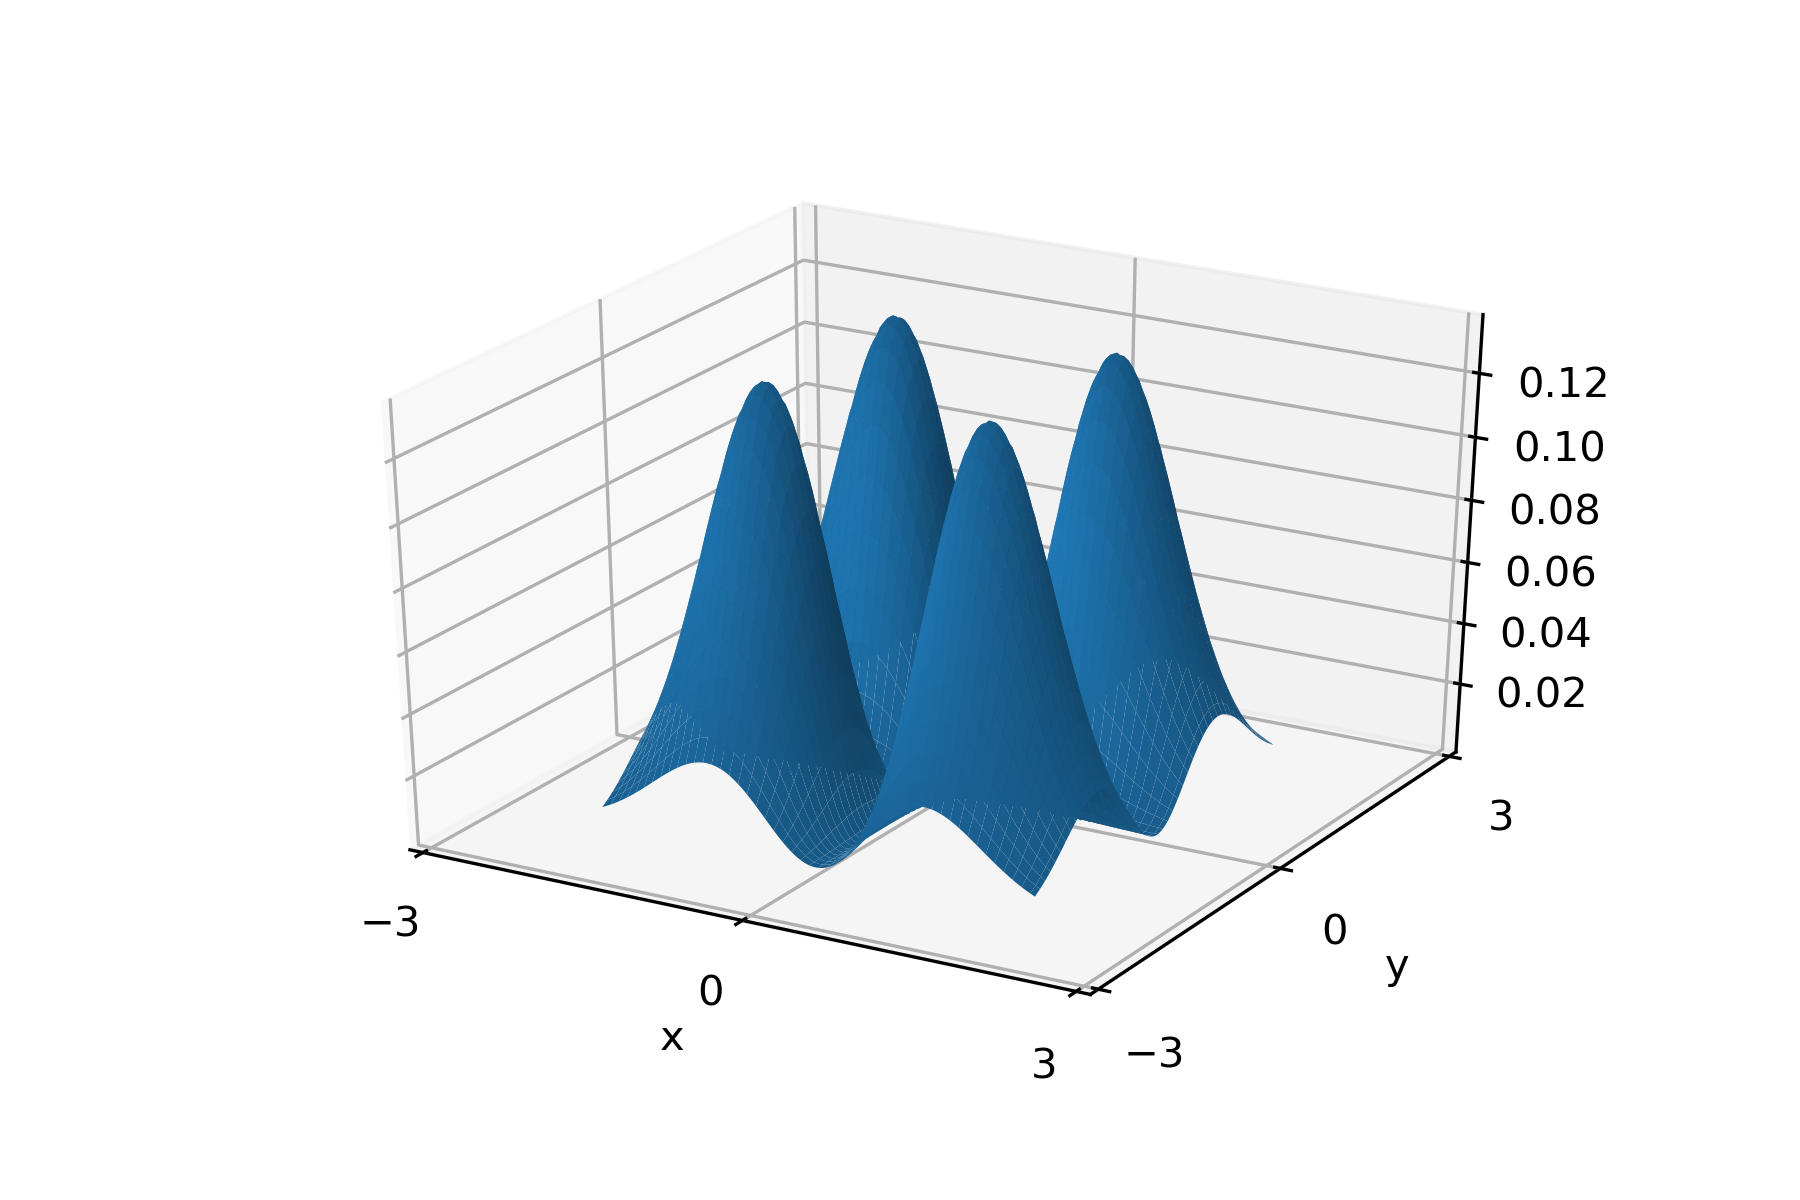
\includegraphics[width=0.66\textwidth]{./four_peaks.png}
	\caption{ $V(x,y) = x^{2}y^{2}e^{-(x^{2}+y^{2})}$ }
\end{figure}

\par The impact parameter is the coordinate $x_{0}$. The initial angle of the
velocity is $\frac{\pi}{2}$ as it points in the direction of the y-axis. The system
is very dependent on the initial speed results in the elimination of the effect of
the potential. I suppose this is due to the fact that the point does not stays enough
in the zone where the potential is the most effective. For didactic purposes I made two
plots showing the chaotic results. Setting $x_{0} \in [0., 5.]$ one can see that
the scattering is chaotic in the $[0. ,1.]$ region. Using 1001 steps and setting the
experiment duration to 1000 seconds and 4001 steps between \textit{[0, 5]} and
\textit{[0, 1]}.

\begin{figure}[H]
	\centering
	\begin{minipage}{0.5\textwidth}
		\centering
		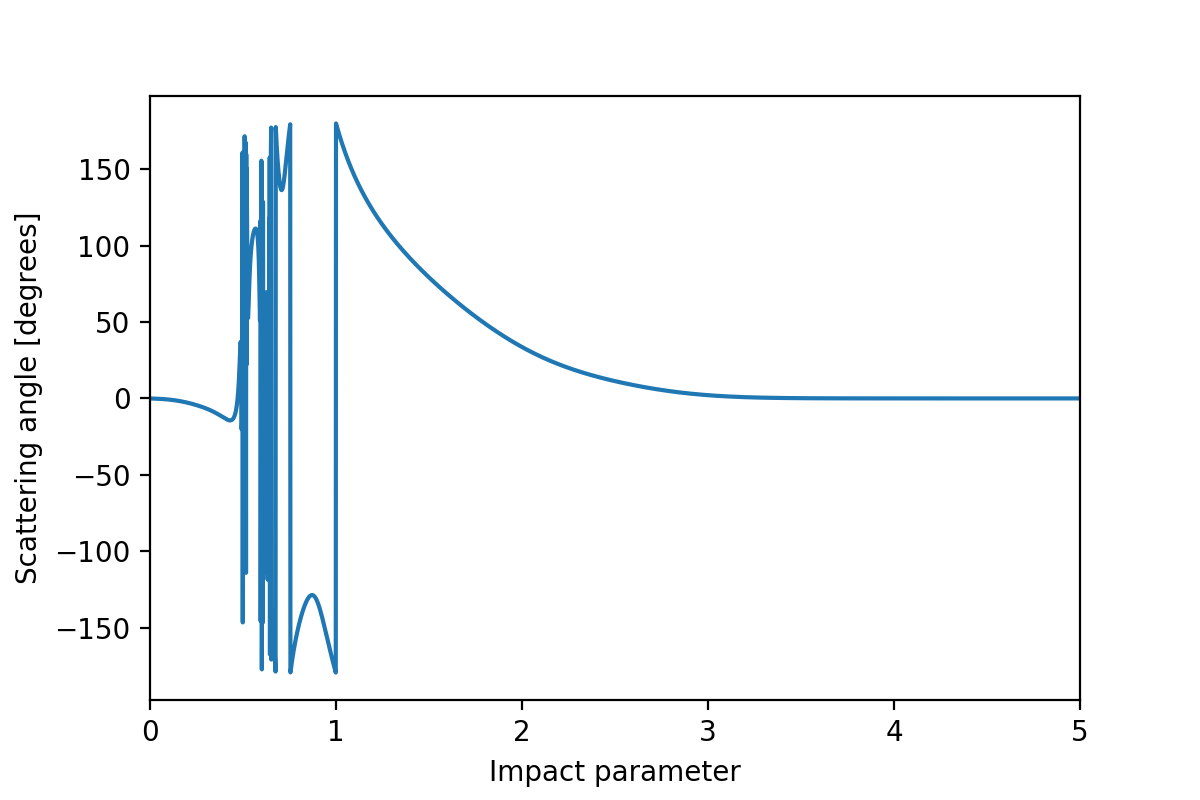
\includegraphics[width=0.95\textwidth]{./chaotic-scattering1.png}
		\caption{ $x_{0} \in [0., 5.]$ }
	\end{minipage}\hfill
	\begin{minipage}{0.5\textwidth}
		\centering
		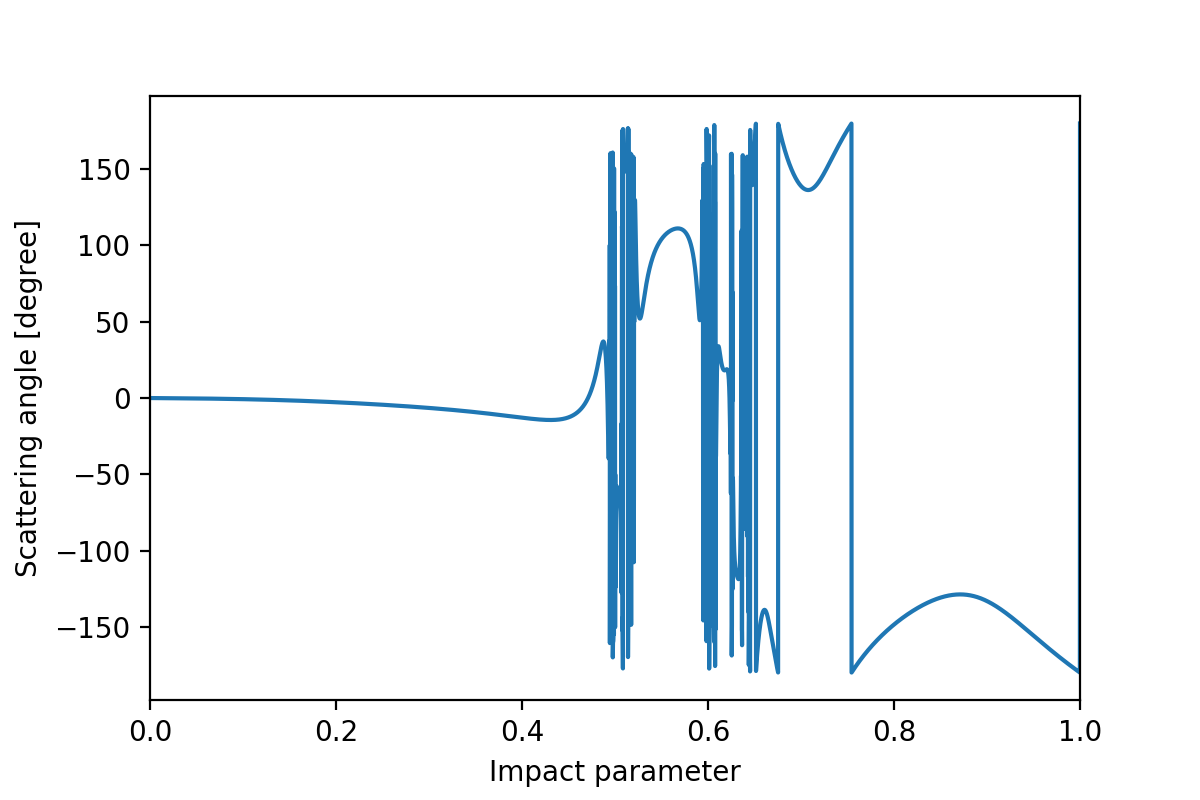
\includegraphics[width=0.95\textwidth]{./chaotic-scattering2.png}
		\caption{$x_{0} \in [0., 1.]$}
	\end{minipage}
\end{figure}

\subsubsection{Book example (-)}

\begin{figure}[H]
	\centering
	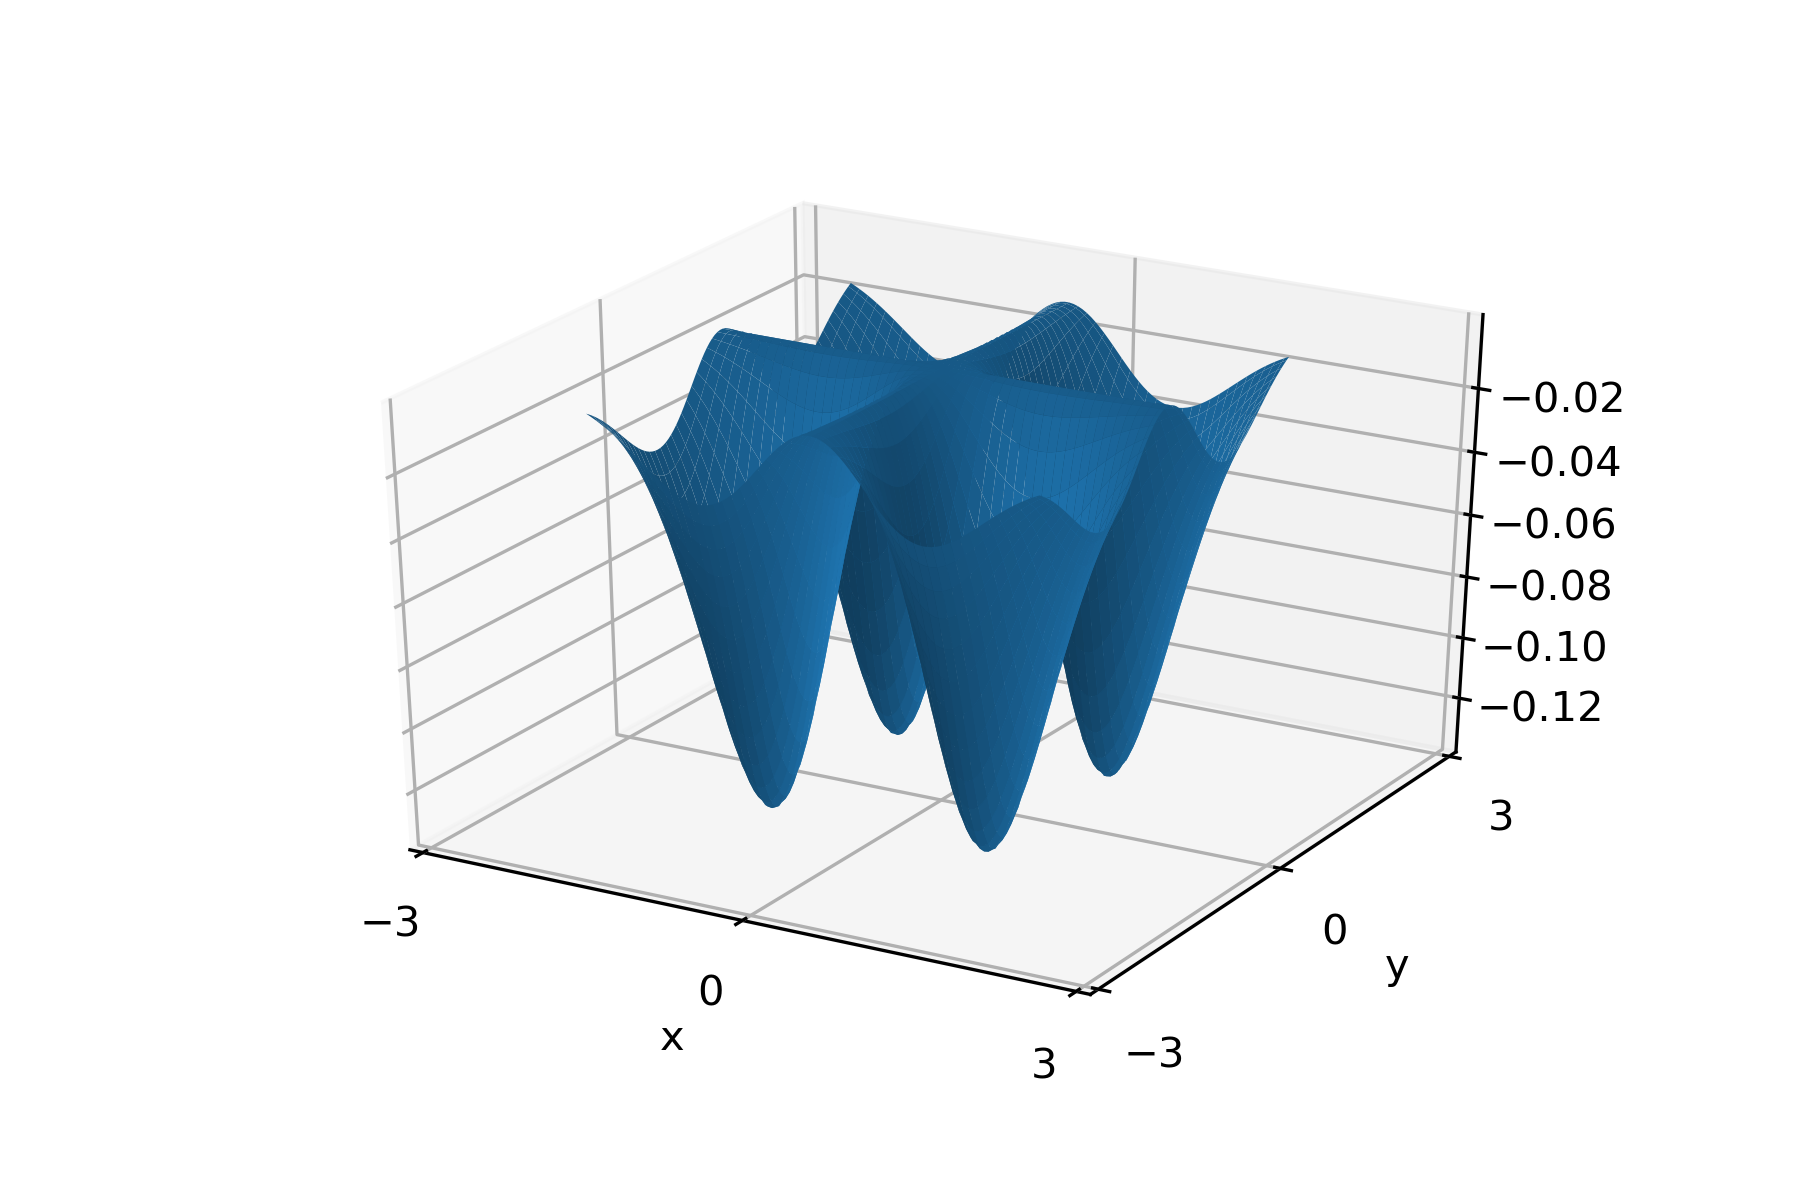
\includegraphics[width=0.66\textwidth]{./four_peaks2.png}
	\caption{ $V(x,y) = -x^{2}y^{2}e^{-(x^{2}+y^{2})}$ }
\end{figure}

\par Using the same parameters as before, only changed the sign of the potential.

\begin{figure}[H]
	\centering
	\begin{minipage}{0.5\textwidth}
		\centering
		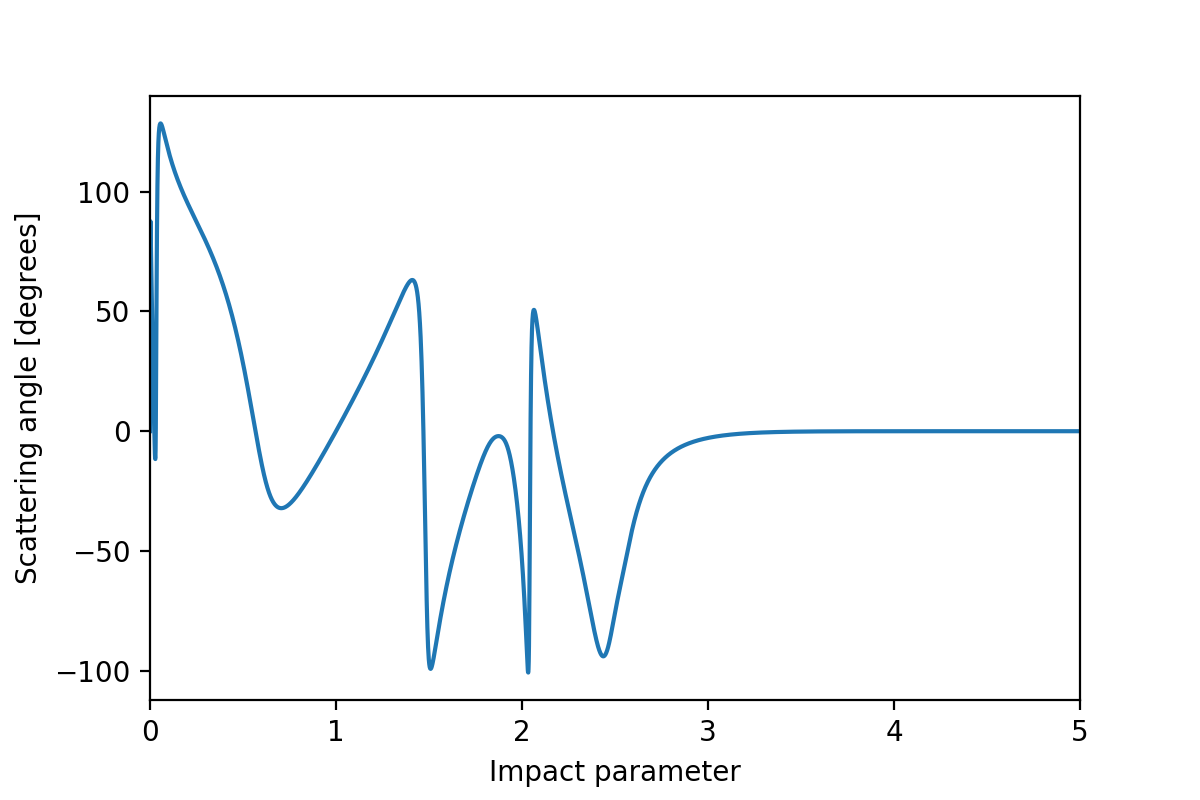
\includegraphics[width=0.95\textwidth]{./chaotic-scattering1signed.png}
        \caption{ $x_{0} \in [0., 5.]$ }
	\end{minipage}\hfill
	\begin{minipage}{0.5\textwidth}
		\centering
		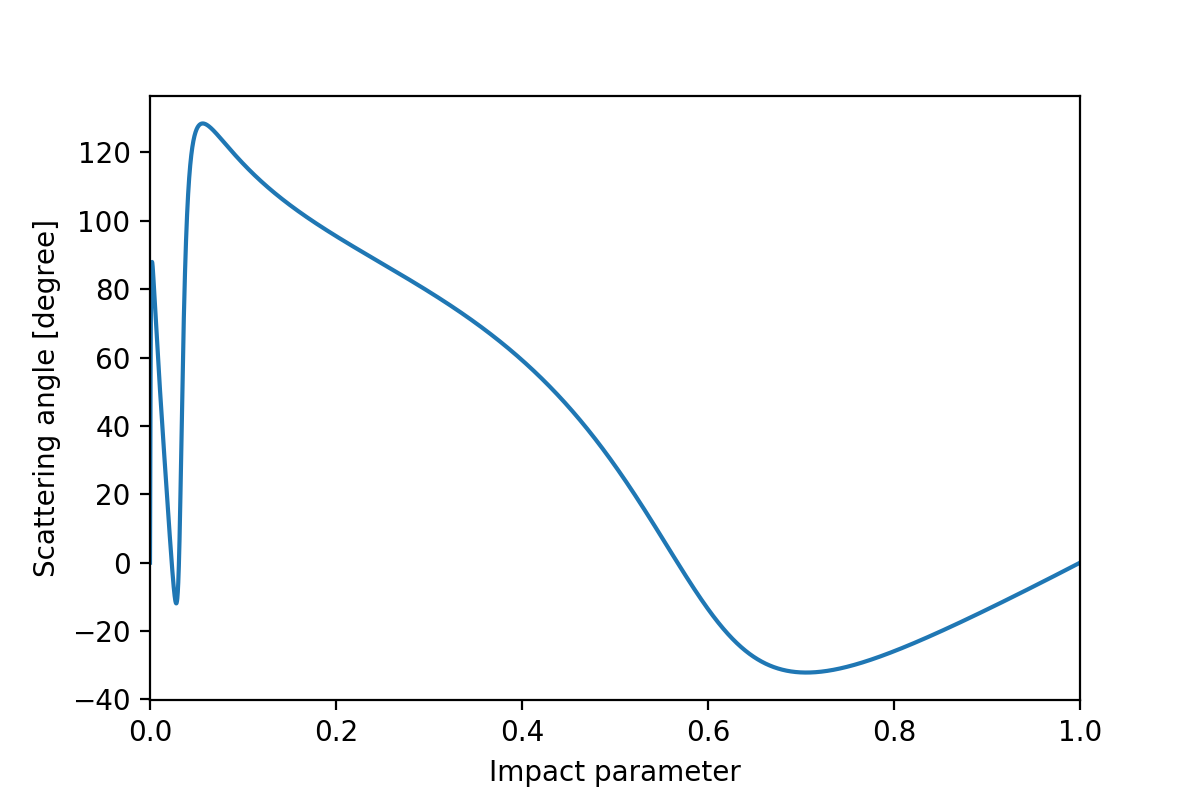
\includegraphics[width=0.95\textwidth]{./chaotic-scattering2signed.png}
		\caption{$x_{0} \in [0., 1.]$}
	\end{minipage}
\end{figure}

\subsubsection{Custom potential (+)/(-)}

\par I used the same constants and methods to do the experiment and the plots. The
previously shown \textit{scatter} function was obviously changed since I needed to
update the potential and its derivatives:

\begin{align*}
	I. \quad m\dot{u}(t) = \mp 2x(1-x^{2})e^{-(x^{2}+y^{2})} \\ \\
	II. \quad m\dot{v}(t) = \pm 2x^{2}ye^{-(x^{2}+y^{2})}
\end{align*}

\begin{figure}[H]
	\centering
	\begin{minipage}{0.5\textwidth}
		\centering
		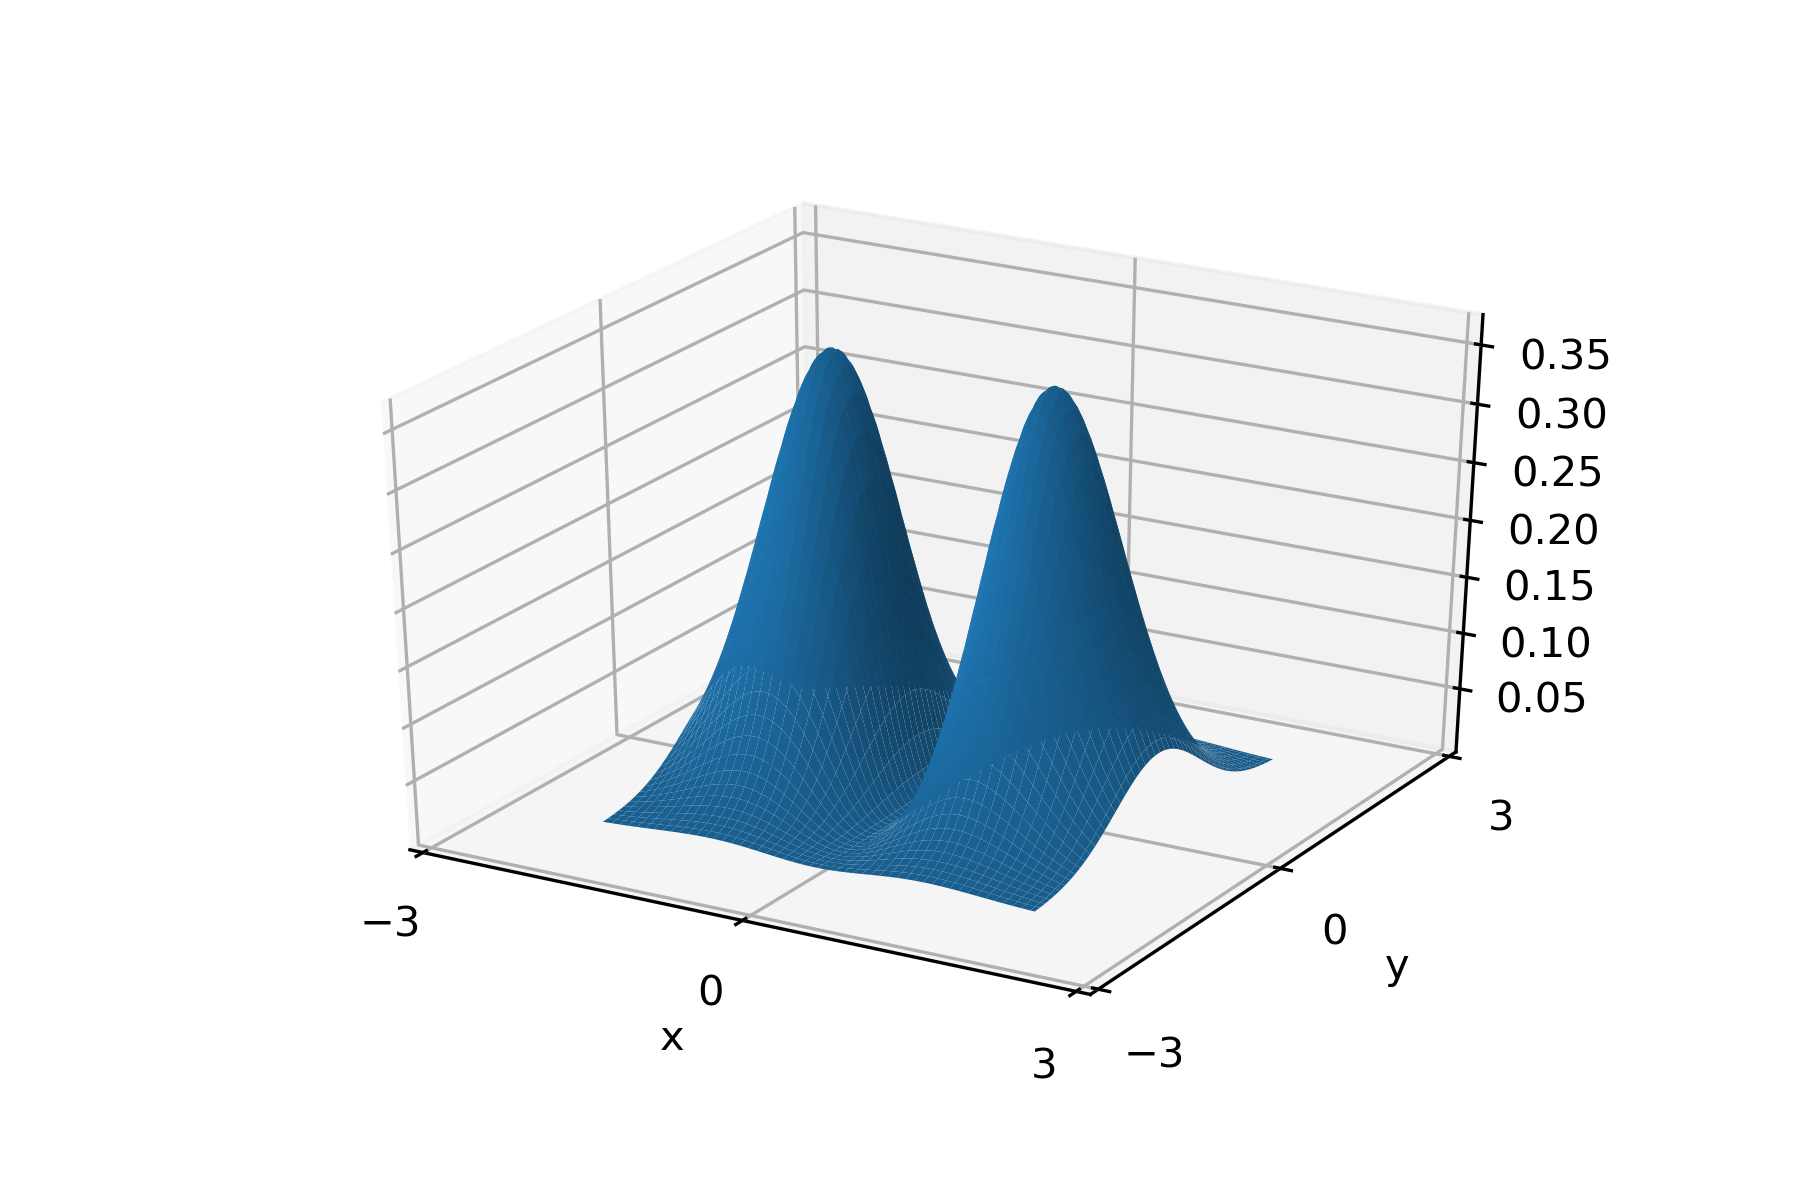
\includegraphics[width=0.96\textwidth]{./two_peaks.png}
		\caption{ $V(x,y) = x^{2}e^{-(x^{2}+y^{2})}$ }
	\end{minipage}\hfill
	\begin{minipage}{0.5\textwidth}
		\centering
		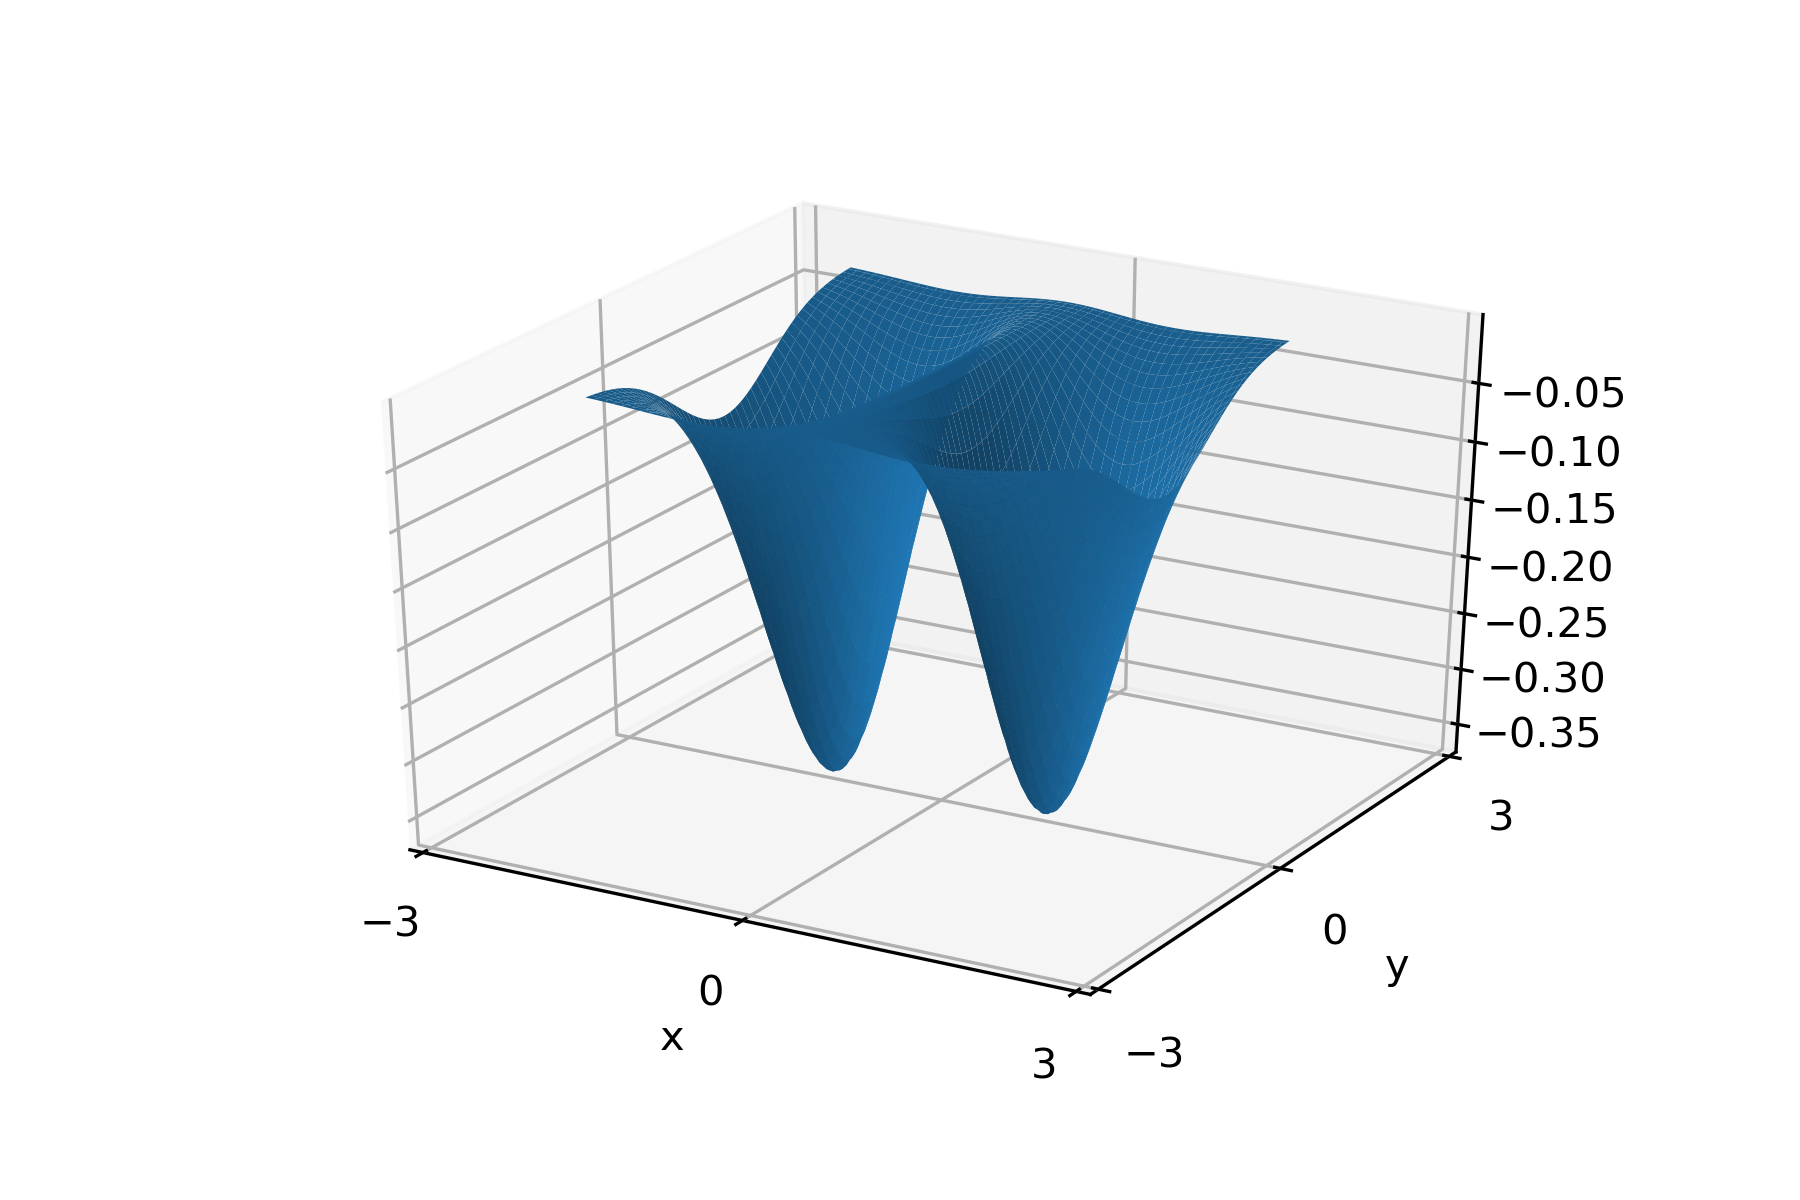
\includegraphics[width=0.96\textwidth]{./two_peaks2.png}
		\caption{ $V(x,y) = -x^{2}e^{-(x^{2}+y^{2})}$ }
	\end{minipage}\hfill
\end{figure}

\par Due to symmetry reasons changing \textbf{x-y} only rotates the potential and therefore
it should not be updated, it can be tested with varying the initial conditions. The results
are shown for both (+) and (-) signed potentials.

\begin{figure}[H]
	\centering
	\begin{minipage}{0.5\textwidth}
		\centering
		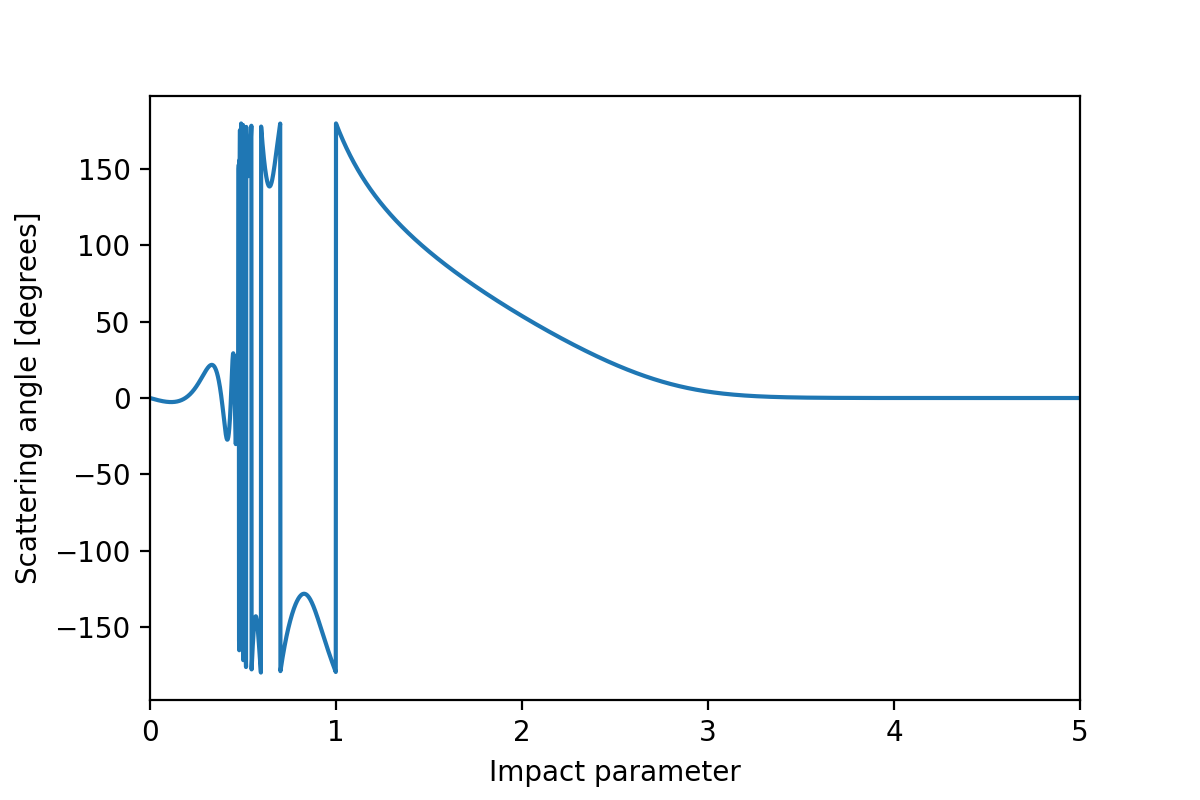
\includegraphics[width=0.95\textwidth]{./chaotic-scattering-co1.png}
		\caption{ (+) $x_{0} \in [0., 5.]$ }
	\end{minipage}\hfill
	\begin{minipage}{0.5\textwidth}
		\centering
		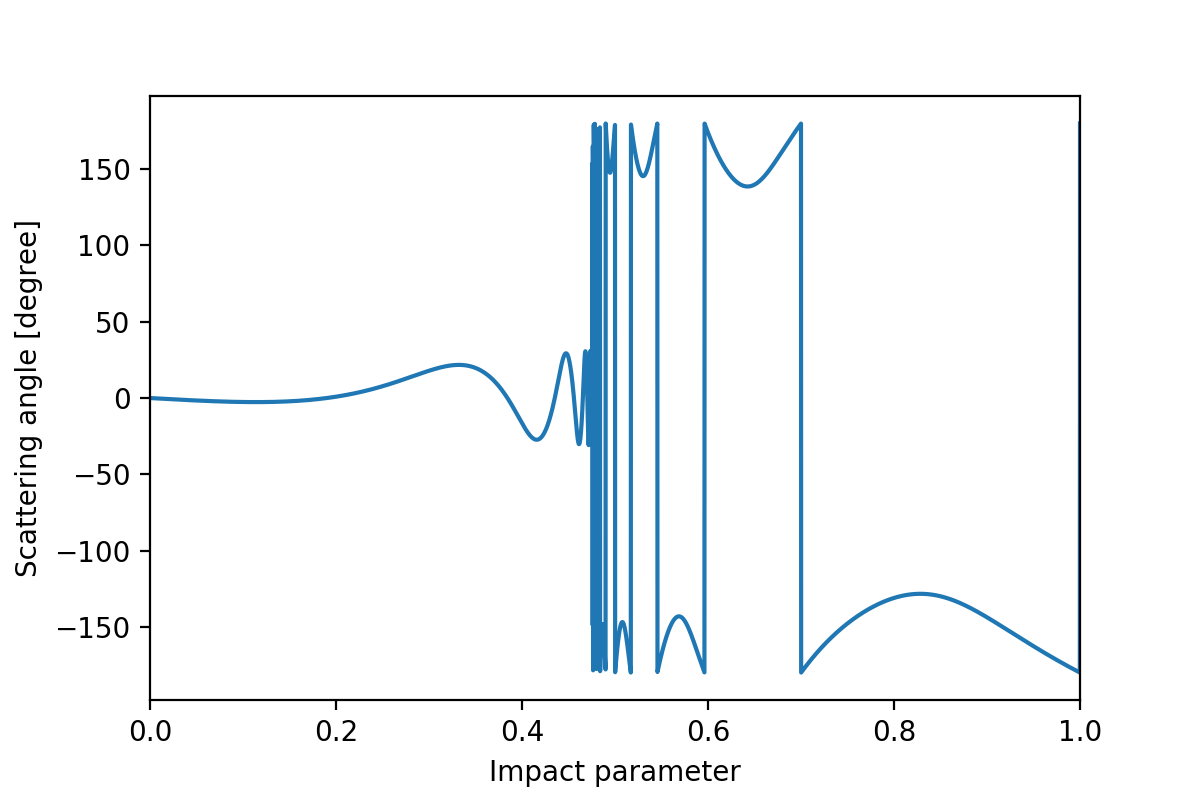
\includegraphics[width=0.95\textwidth]{./chaotic-scattering-co2.png}
		\caption{ (+) $x_{0} \in [0., 1.]$}
	\end{minipage}
\end{figure}

\begin{figure}[H]
	\centering
	\begin{minipage}{0.5\textwidth}
		\centering
		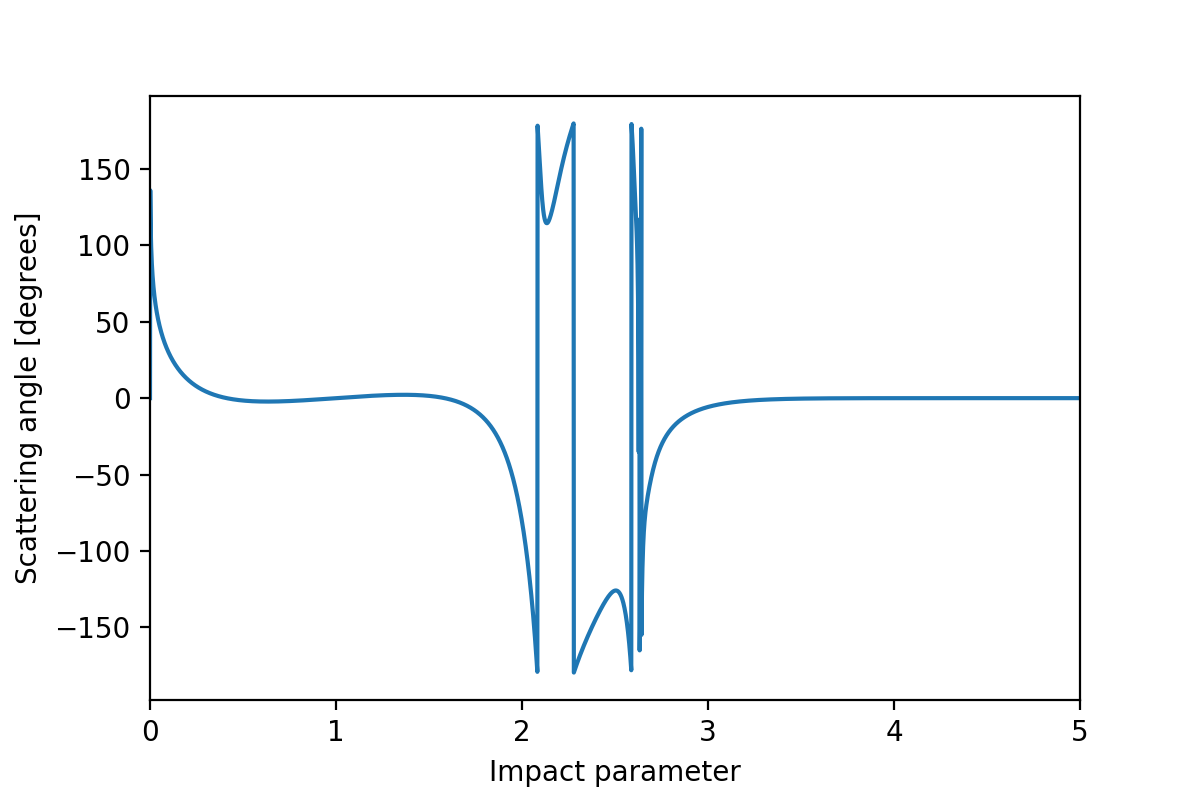
\includegraphics[width=0.95\textwidth]{./chaotic-scattering-co1signed.png}
		\caption{ (-) $x_{0} \in [0., 5.]$ }
	\end{minipage}\hfill
	\begin{minipage}{0.5\textwidth}
		\centering
		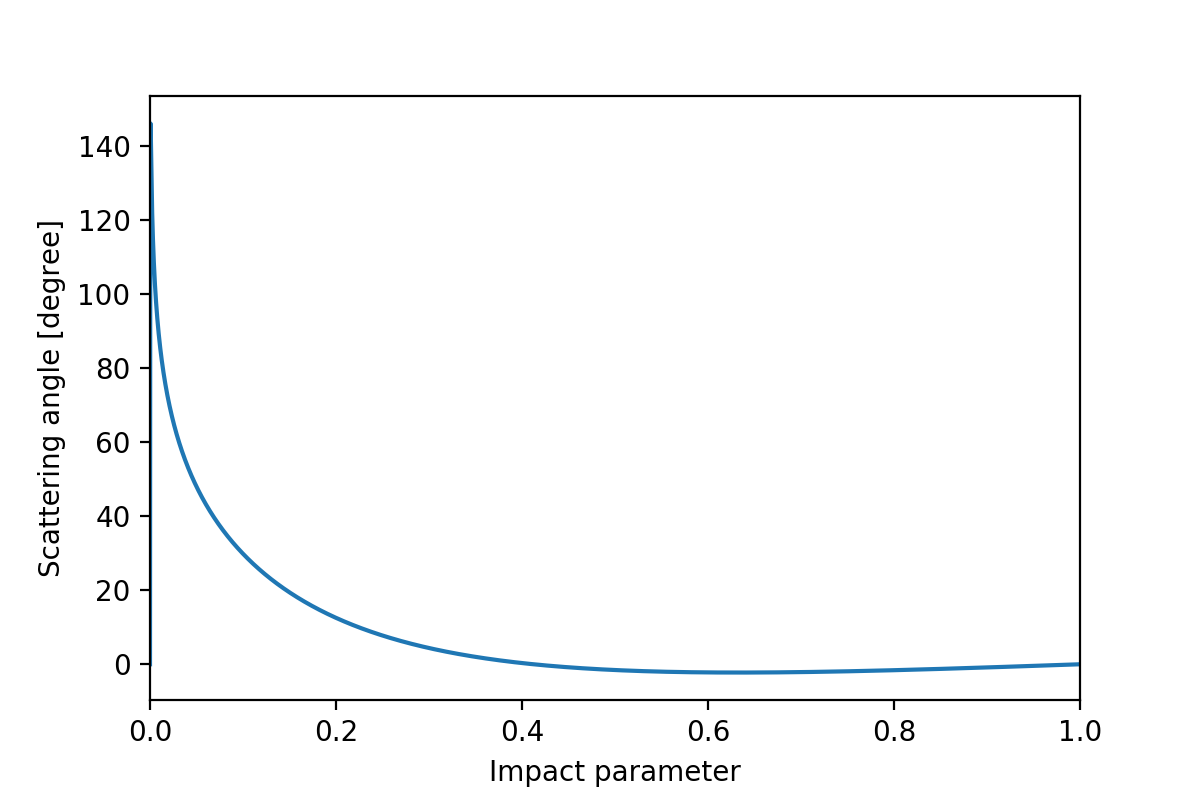
\includegraphics[width=0.95\textwidth]{./chaotic-scattering-co2signed.png}
		\caption{ (-) $x_{0} \in [0., 1.]$}
	\end{minipage}
\end{figure}

\section{The cross section}

\par Using the acquired impact parameters and  of course the acquired angles the
cross section is the following function:

\begin{equation}
	\sigma(\vartheta) = \Big|\frac{d\vartheta}{db}\Big|\frac{b}{sin(\vartheta)}
\end{equation}

\par The derivative of theta could be easilly acquired by calculating:

\begin{equation}
	\frac{d\vartheta}{db} \approx \frac{\Delta \vartheta}{\Delta b} = \frac{\vartheta_{i+1} - \vartheta_{i}}{\Delta b}
\end{equation}

\par Acquiring the set from the outputted data $b, \vartheta$ I calculated the cross section
for each potential for all signs.

\par The following cross sections were acquired:

\subsection{Potentials}

\subsubsection{Book example (+)/(-)}

\begin{figure}[H]
	\centering
	\begin{minipage}{0.5\textwidth}
		\centering
		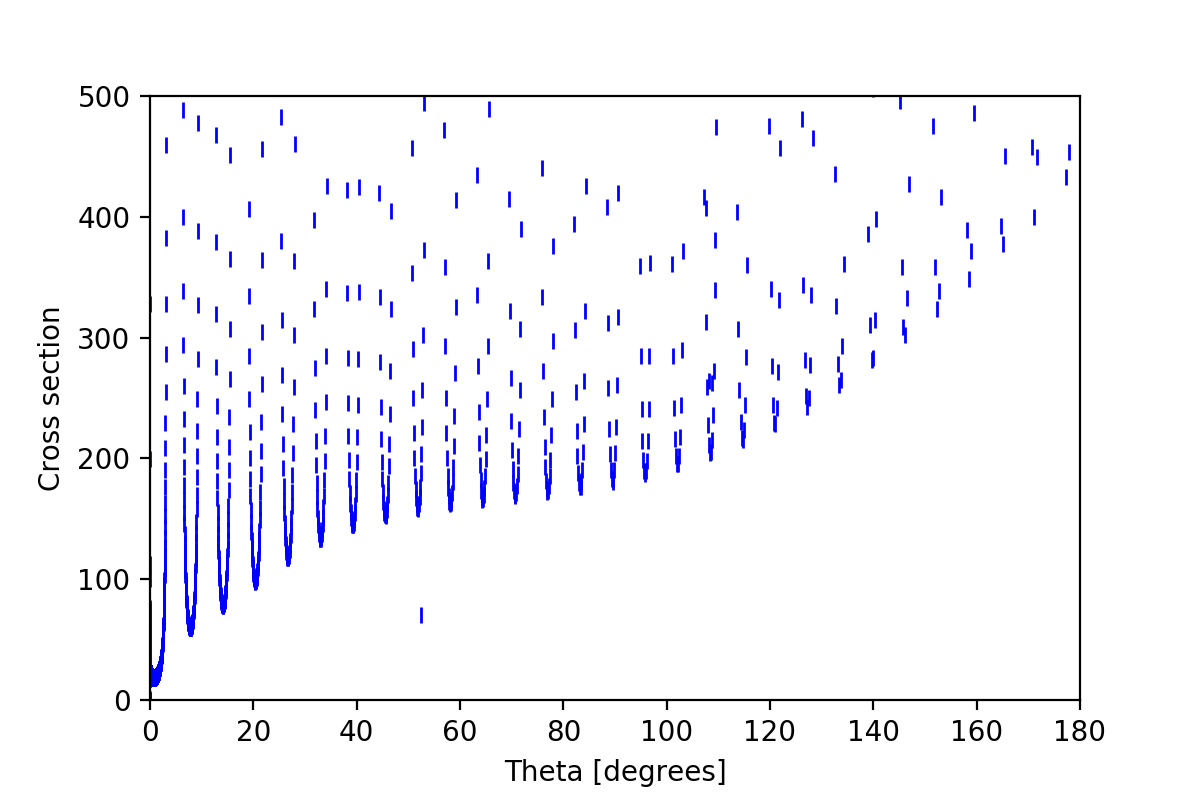
\includegraphics[width=0.95\textwidth]{./cross-pot-og1.png}
		\caption{ (+) $\vartheta \in [0., 180.]$ }
	\end{minipage}\hfill
	\begin{minipage}{0.5\textwidth}
		\centering
		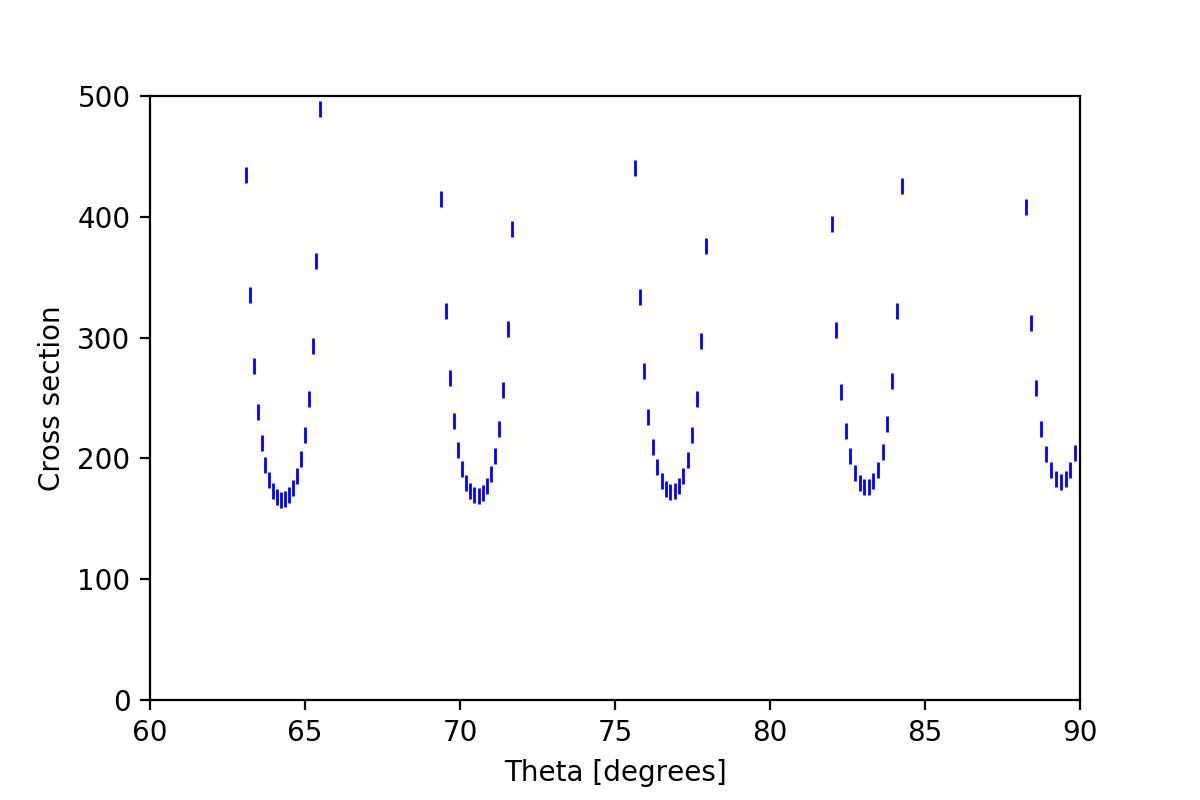
\includegraphics[width=0.95\textwidth]{./cross-pot-og2.png}
		\caption{ (+) $\vartheta \in [60., 90.]$}
	\end{minipage}
\end{figure}

\begin{figure}[H]
	\centering
	\begin{minipage}{0.5\textwidth}
		\centering
		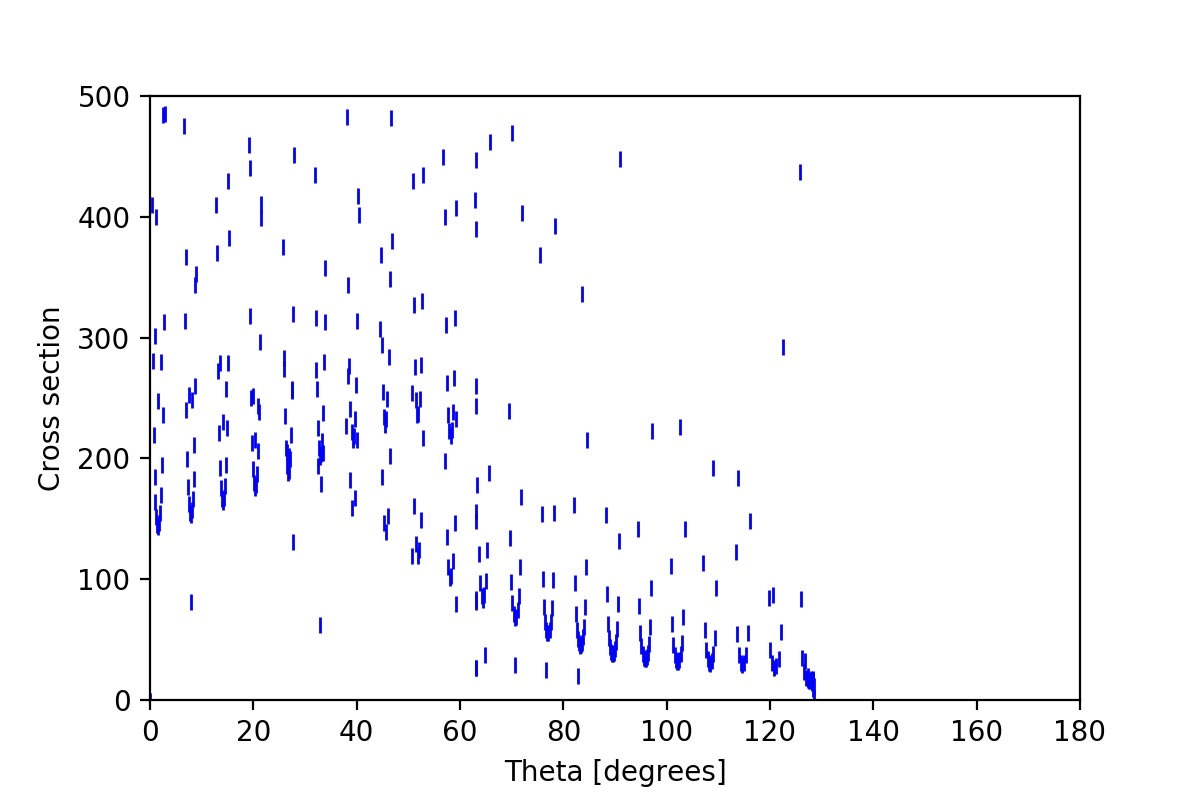
\includegraphics[width=0.95\textwidth]{./cross-pot-og1signed.png}
		\caption{ (-) $\vartheta \in [0., 180.]$ }
	\end{minipage}\hfill
	\begin{minipage}{0.5\textwidth}
		\centering
		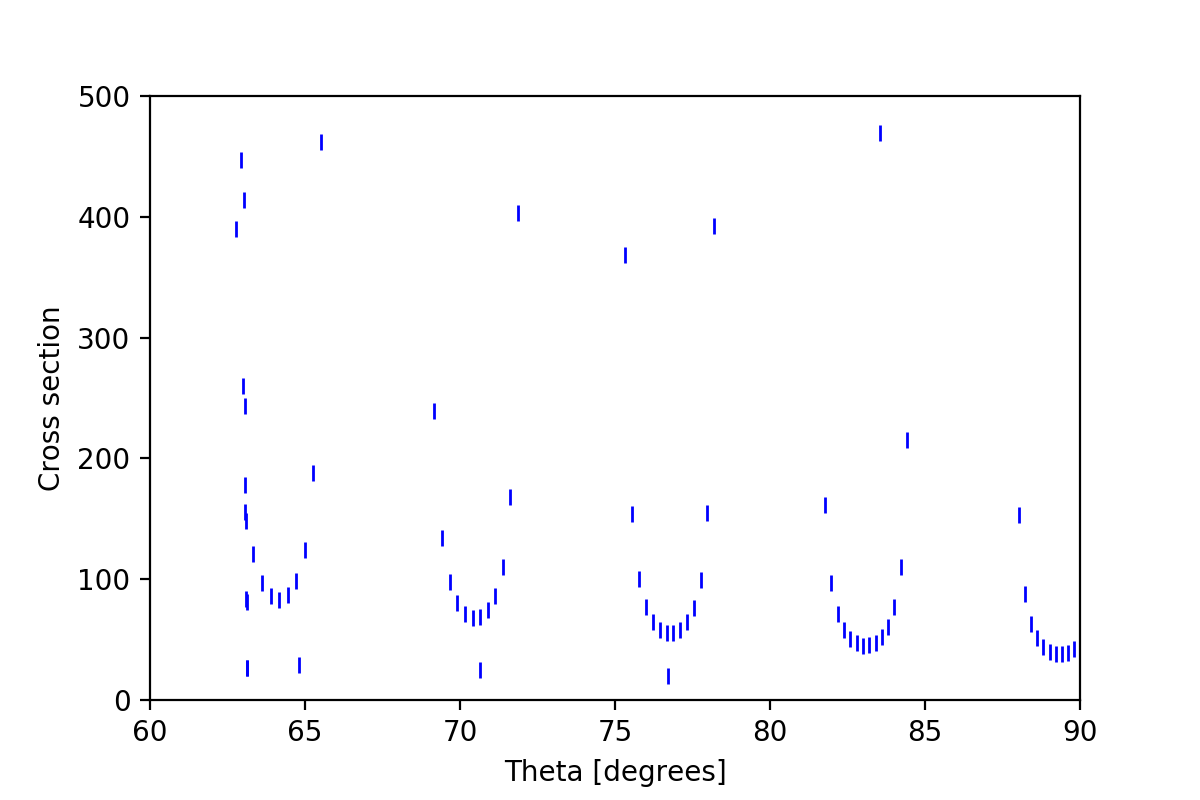
\includegraphics[width=0.95\textwidth]{./cross-pot-og2signed.png}
		\caption{ (-) $\vartheta \in [60., 90.]$ }
	\end{minipage}
\end{figure}

\subsubsection{Custom (+)/(-)}

\begin{figure}[H]
	\centering
	\begin{minipage}{0.5\textwidth}
		\centering
		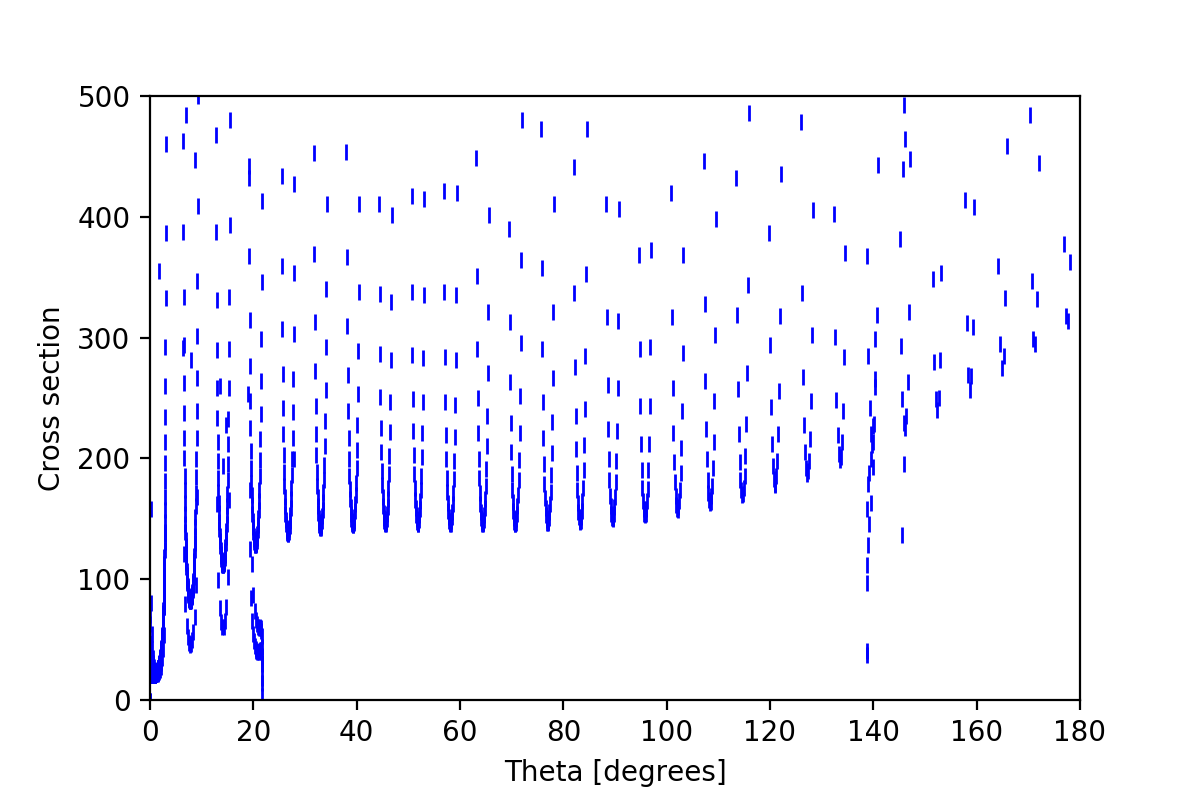
\includegraphics[width=0.95\textwidth]{./cross-pot-co1.png}
		\caption{ (+) $\vartheta \in [0., 180.]$ }
	\end{minipage}\hfill
	\begin{minipage}{0.5\textwidth}
		\centering
		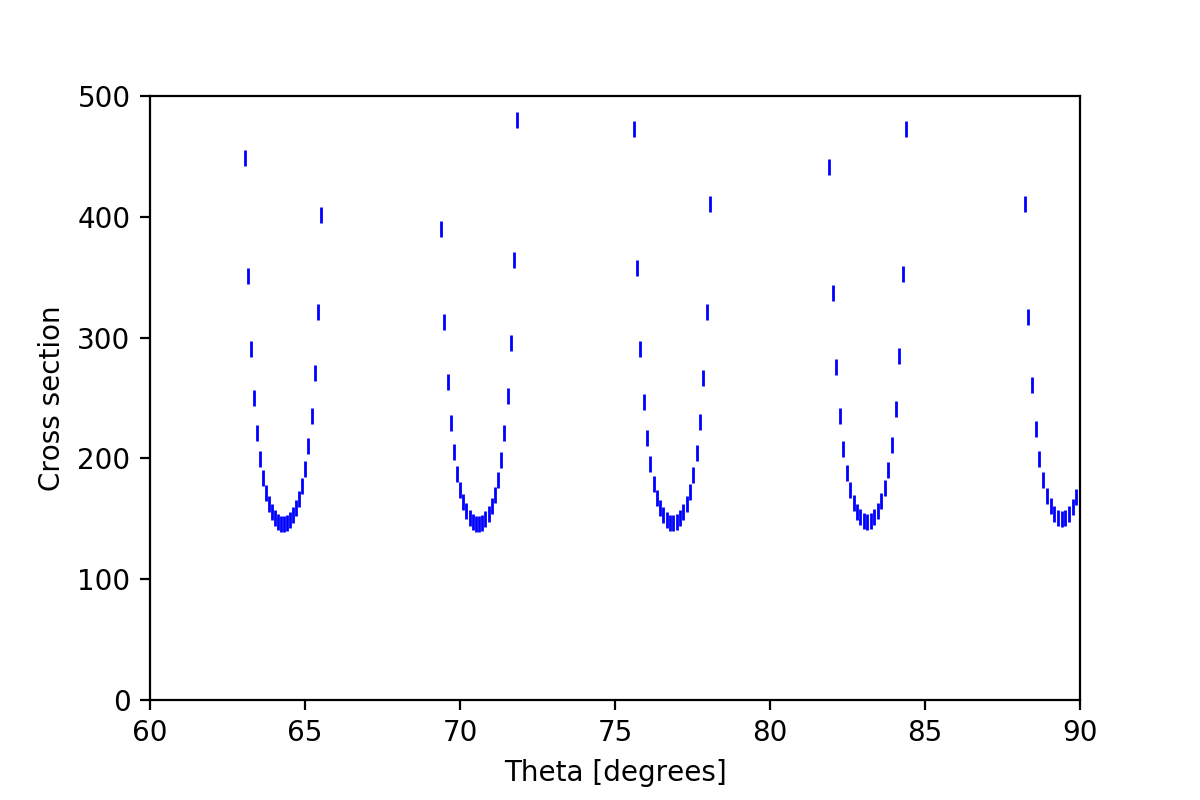
\includegraphics[width=0.95\textwidth]{./cross-pot-co2.png}
		\caption{ (+) $\vartheta \in [60., 90.]$}
	\end{minipage}
\end{figure}

\begin{figure}[H]
	\centering
	\begin{minipage}{0.5\textwidth}
		\centering
		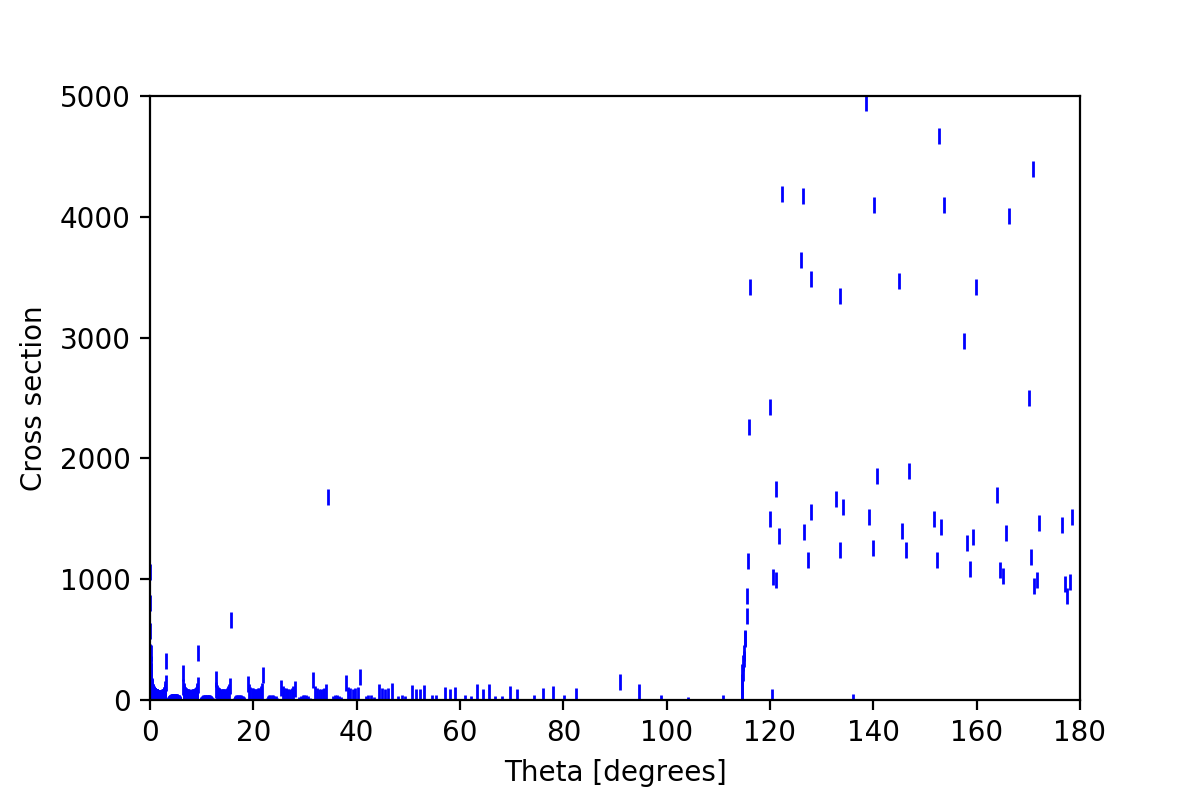
\includegraphics[width=0.95\textwidth]{./cross-pot-co1signed.png}
		\caption{ (-) $\vartheta \in [0., 180.]$ }
	\end{minipage}\hfill
	\begin{minipage}{0.5\textwidth}
		\centering
		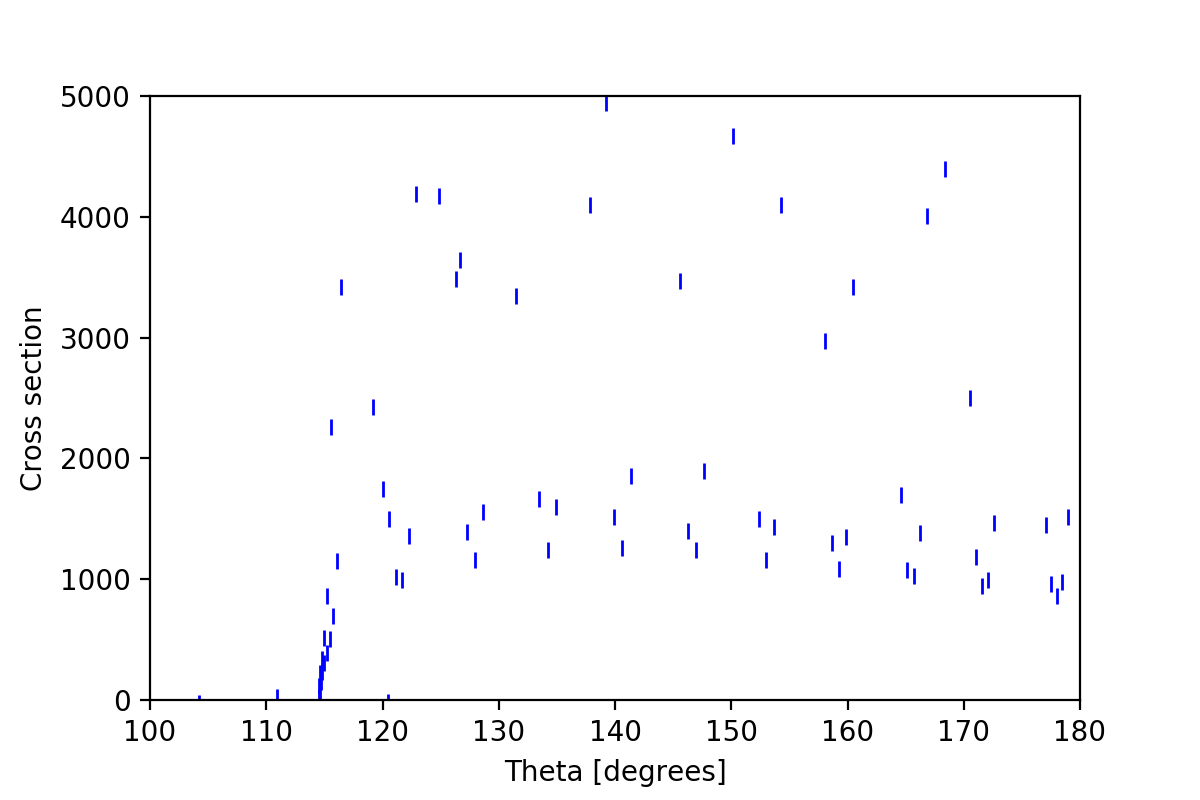
\includegraphics[width=0.95\textwidth]{./cross-pot-co2signed.png}
		\caption{ (-) $\vartheta \in [100., 180.]$ }
	\end{minipage}
\end{figure}

\subsection{Interpretation}

\par I wish I could give a satisfactory explanation to
the cross sections seen above, however I cannot. I can
check them qualitatively though. It can be seen clearly that
for attractive potentials the cross section is getting smaller as
the scattering angle gets bigger, this is due to the fact that
I calculated the \textit{atan2} of $v_y, v_x$ and not the other way
around, but the trend is trivially there. For repressive
potentials the cross section is much higher in the angles under
(inverse degree scale again) 90 degrees, this can be regarded as
back scattering.

\section{Phase space diagrams}

\par For one scattering, only for visualization:

\subsection{Potentials}

\subsubsection{Book example (+)/(-)}

\begin{figure}[H]
	\centering
	\begin{minipage}{0.5\textwidth}
		\centering
		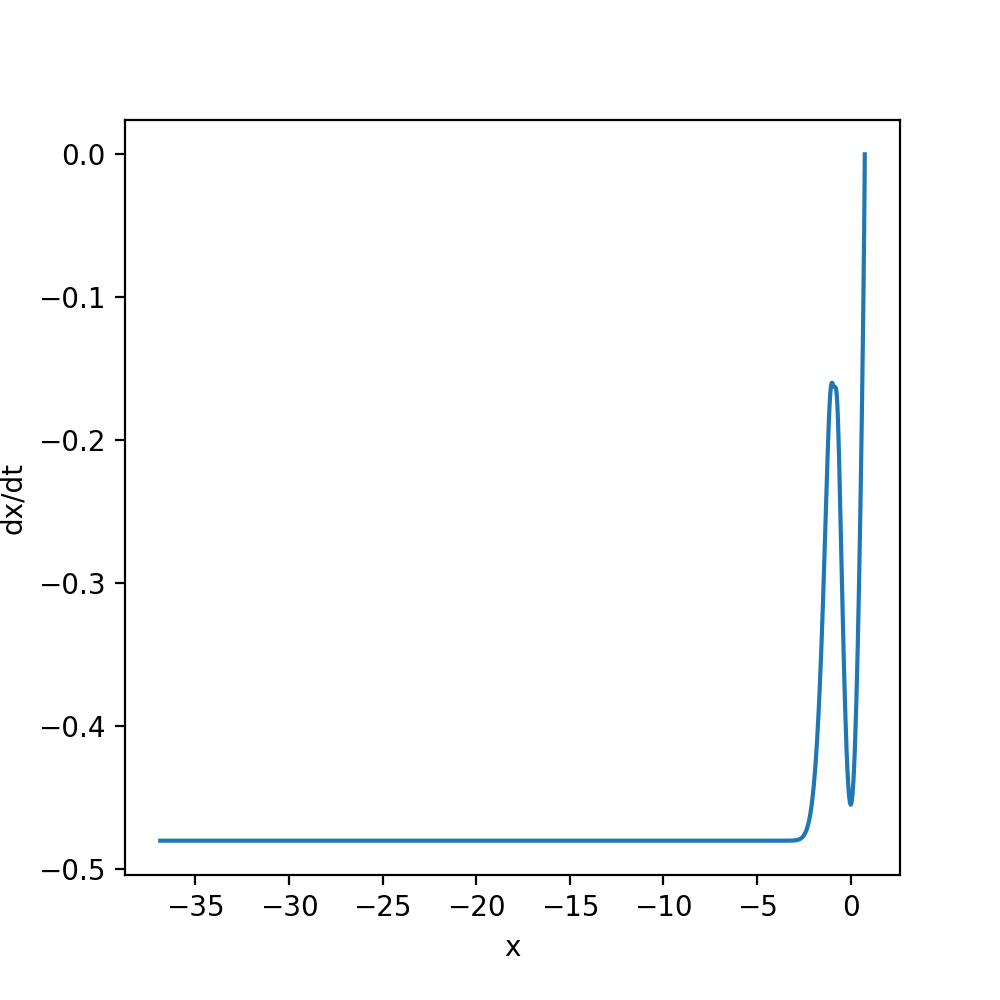
\includegraphics[width=0.95\textwidth]{./phase-og-1.png}
		\caption{ (+) $x(t), \dot{x}(t)$ }
	\end{minipage}\hfill
	\begin{minipage}{0.5\textwidth}
		\centering
		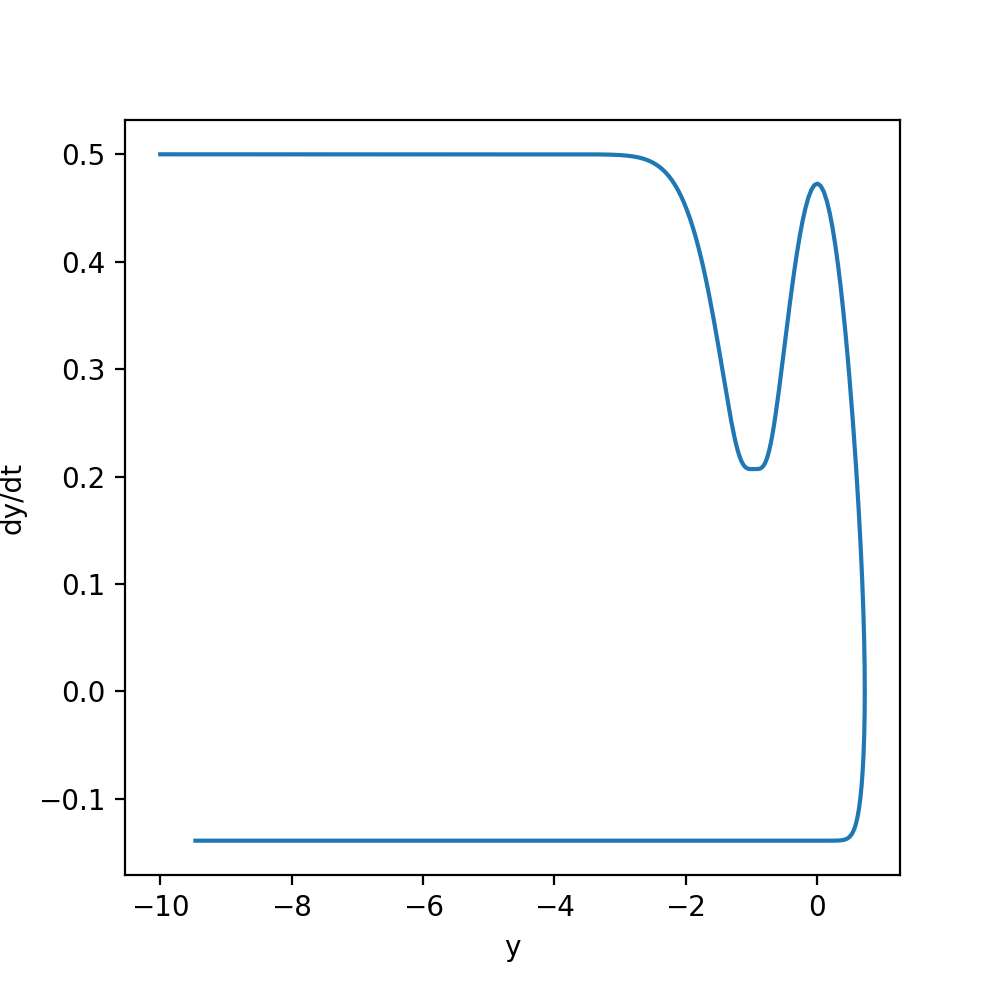
\includegraphics[width=0.95\textwidth]{./phase-og-2.png}
		\caption{ (+) $y(t), \dot{y}(t)$ }
	\end{minipage}
\end{figure}

\begin{figure}[H]
	\centering
	\begin{minipage}{0.5\textwidth}
		\centering
		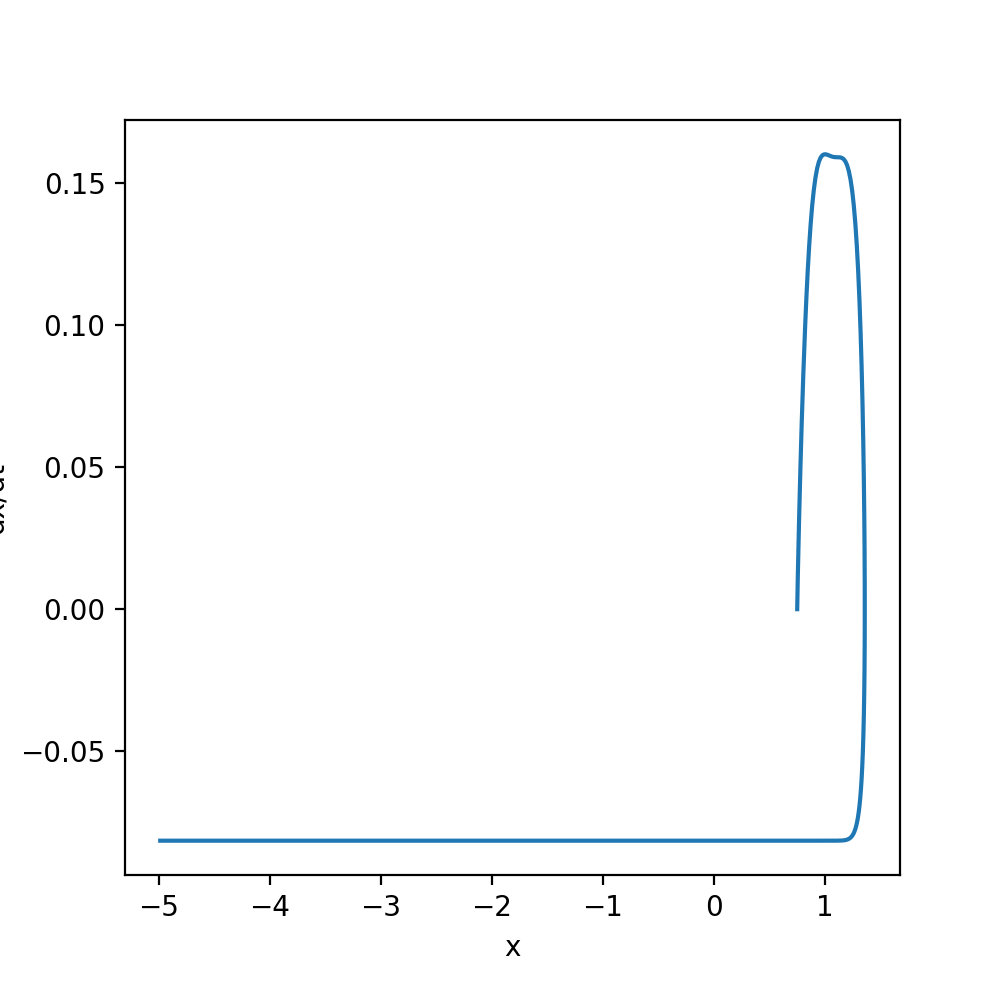
\includegraphics[width=0.95\textwidth]{./phase-og-1signed.png}
		\caption{ (-) $x(t), \dot{x}(t)$ }
	\end{minipage}\hfill
	\begin{minipage}{0.5\textwidth}
		\centering
		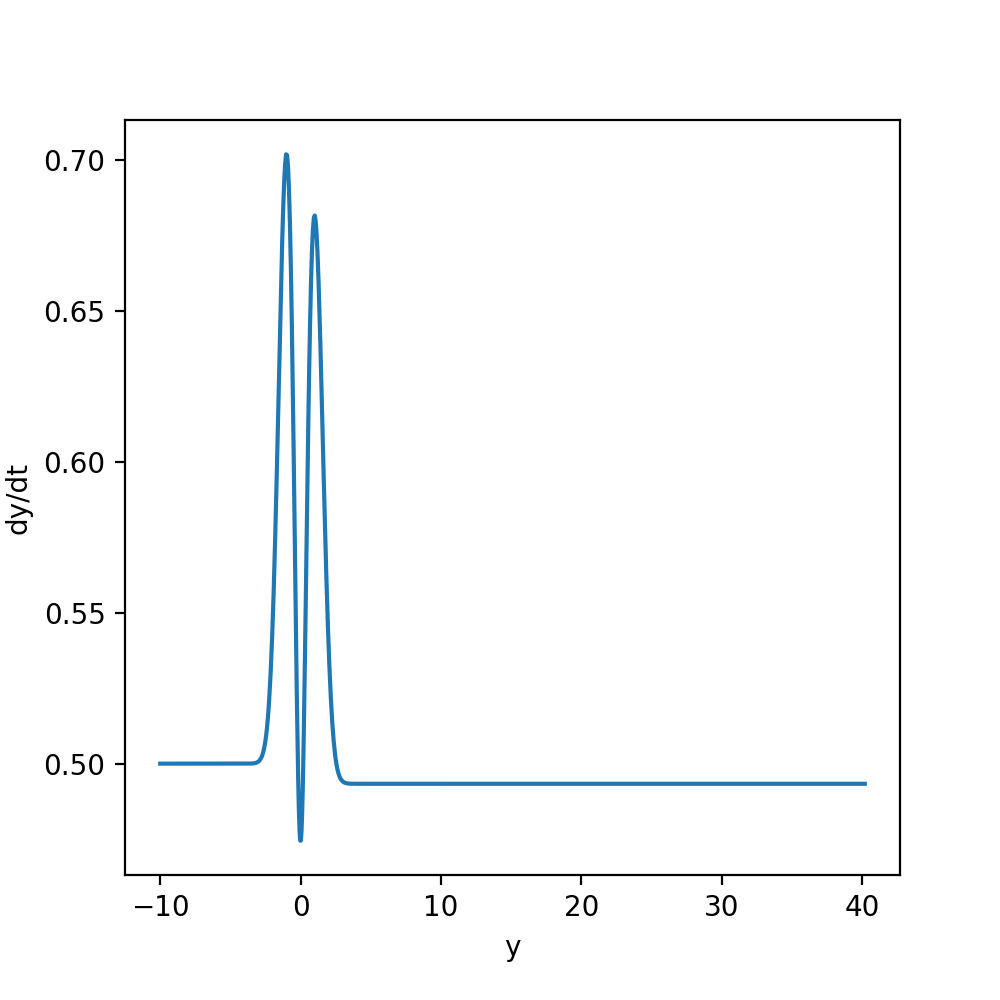
\includegraphics[width=0.95\textwidth]{./phase-og-2signed.png}
		\caption{ (-) $y(t), \dot{y}(t)$ }
	\end{minipage}
\end{figure}

\subsubsection{Custom example (+)/(-)}

\begin{figure}[H]
	\centering
	\begin{minipage}{0.5\textwidth}
		\centering
		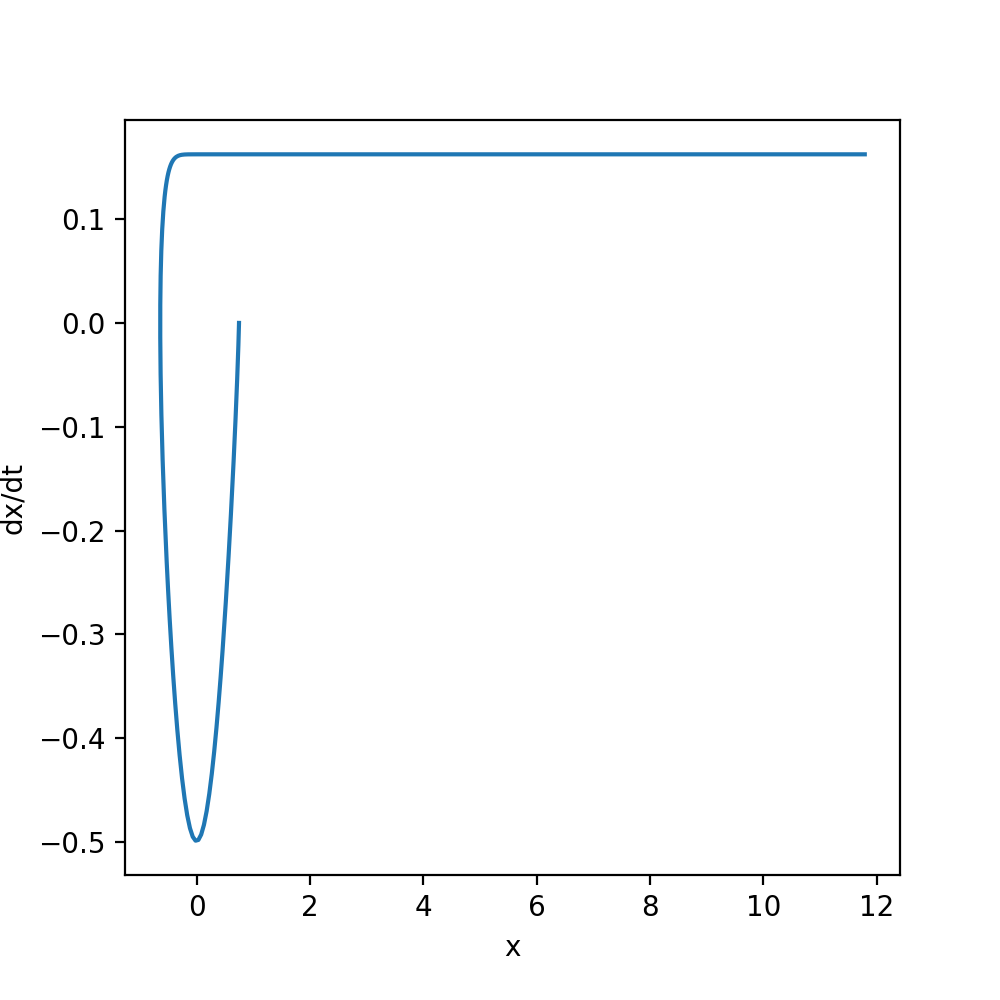
\includegraphics[width=0.95\textwidth]{./phase-og-3.png}
		\caption{ (+) $x(t), \dot{x}(t)$ }
	\end{minipage}\hfill
	\begin{minipage}{0.5\textwidth}
		\centering
		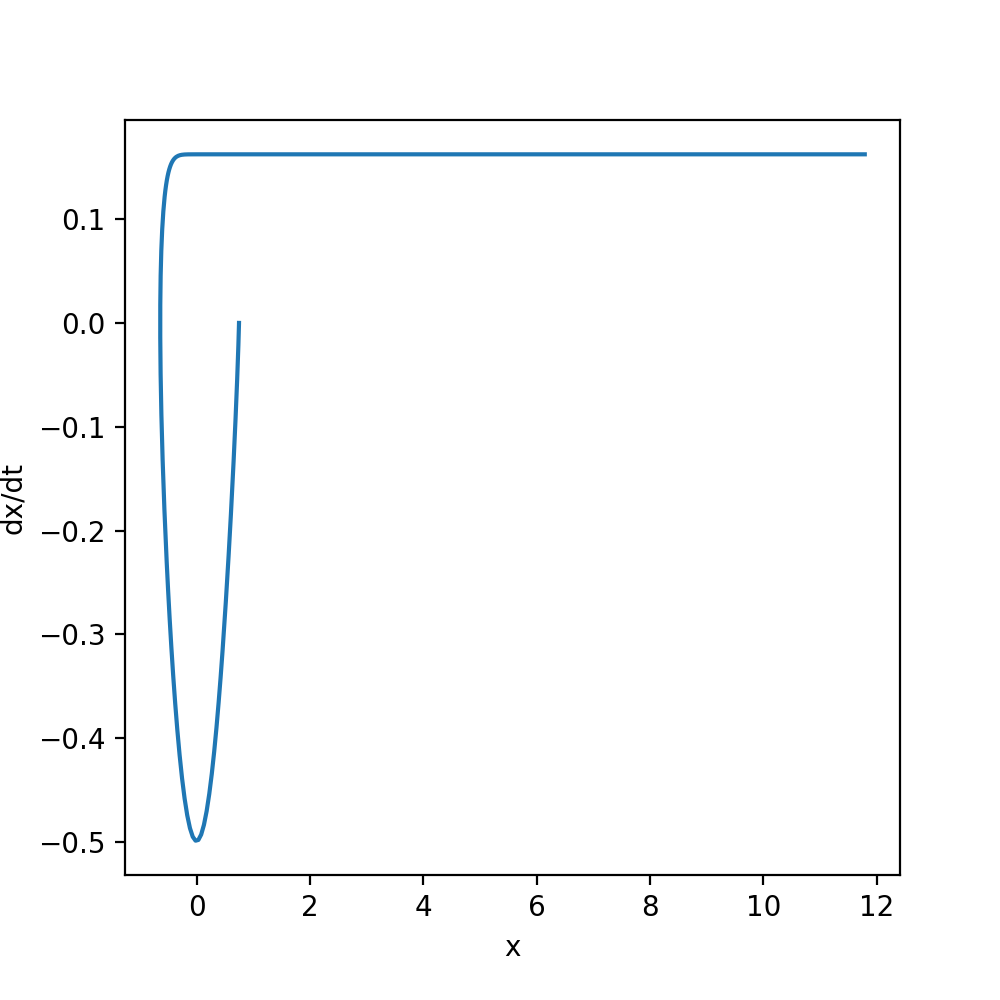
\includegraphics[width=0.95\textwidth]{./phase-og-3.png}
		\caption{ (+) $y(t), \dot{y}(t)$ }
	\end{minipage}
\end{figure}

\begin{figure}[H]
	\centering
	\begin{minipage}{0.5\textwidth}
		\centering
		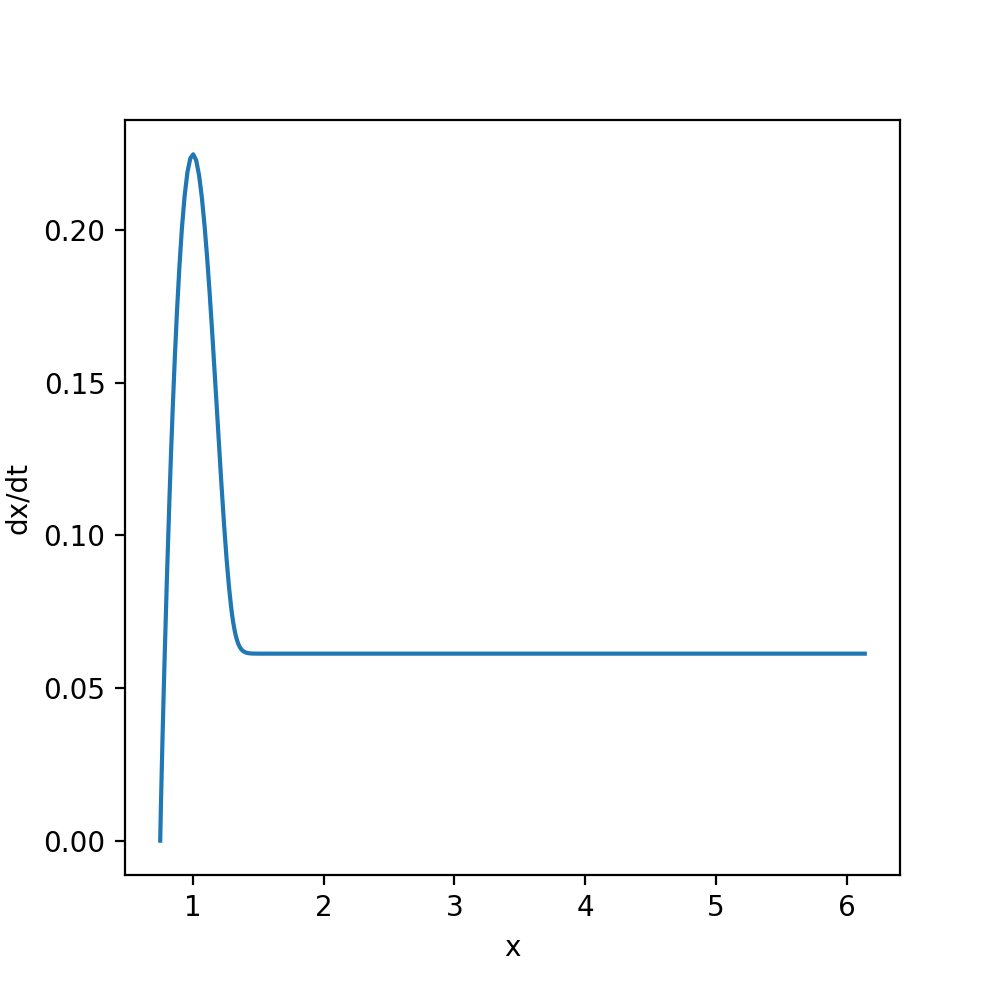
\includegraphics[width=0.95\textwidth]{./phase-og-3signed.png}
		\caption{ (-) $x(t), \dot{x}(t)$ }
	\end{minipage}\hfill
	\begin{minipage}{0.5\textwidth}
		\centering
		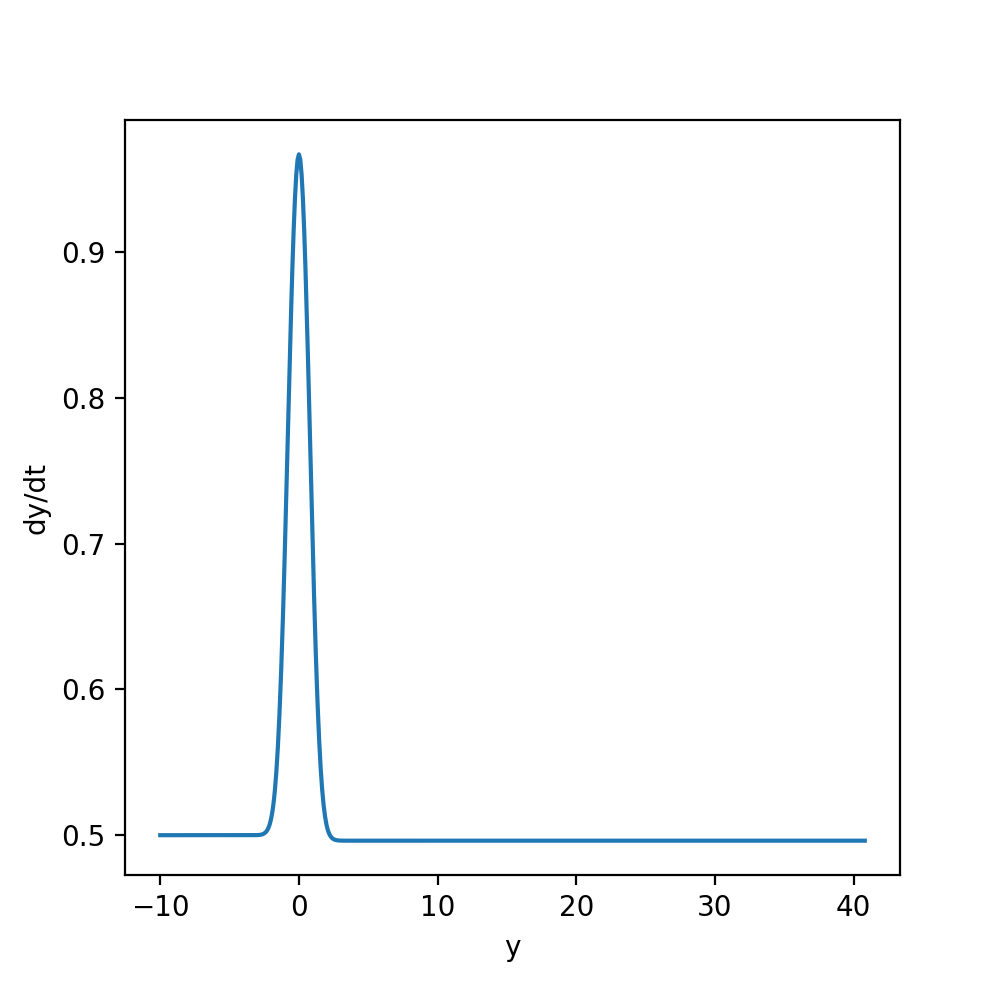
\includegraphics[width=0.95\textwidth]{./phase-og-4signed.png}
		\caption{ (-) $y(t), \dot{y}(t)$ }
	\end{minipage}
\end{figure}

\section{ Overview}

\par I solved the differential equation system efficiently using the
odeint solver \cite{odeint}, although I have not tried different methods I am sure
that real improvement can't be done for that.

\par However, I am certain that my cross section calculations are not the
best, they could be improved by calculating much smaller regions for the impact
parameter and concatenating the results. It can even be parallerized since
the computation does not require to access the same memory regions.

\par There are computational errors evidently as I am dividing by sign
of unknown parameters, therefore I am sometimes dividing by zero, luckily
numpy took care of that efficiently.

\par For attractive potentials there must be some kind error that I
have missed since my results seem wrong.

\par My code is attached at the end with a link pointing to my GitHub
repository \cite{repo}.

\bibliographystyle{plain}
\bibliography{references}

\end{document}